\documentclass[draft]{agujournal2019}

\usepackage{url} %this package should fix any errors with URLs in refs.
% \usepackage{lineno}
\usepackage{amsmath,amssymb}
\usepackage[inline]{trackchanges} %for better track changes. finalnew option will compile document with changes incorporated.
\usepackage{soul}
\usepackage{setspace}
\usepackage{microtype}
\usepackage{silence}
\WarningFilter{latex}{Overfull}
\WarningFilter{latex}{Underfull}
\emergencystretch=3em
\hbadness=10000
\hfuzz=100pt

\relpenalty=10000
\binoppenalty=10000
\thinmuskip=3mu
\medmuskip=4mu
\thickmuskip=5mu
\mathsurround=0pt
\microtypesetup{expansion=false}

\setstretch{1.5}
\newcommand{\citeg}[1]{\cite<e.g.,>[]{#1}}
\newcommand{\citef}[1]{\cite<c.f.,>[]{#1}}
% \linenumbers

%%%%%%%
% As of 2018 we recommend use of the TrackChanges package to mark revisions.
% The trackchanges package adds five new LaTeX commands:
%
%  \note[editor]{The note}
%  \annote[editor]{Text to annotate}{The note}
%  \add[editor]{Text to add}
%  \remove[editor]{Text to remove}
%  \change[editor]{Text to remove}{Text to add}
%
% complete documentation is here: http://trackchanges.sourceforge.net/
%%%%%%%

\draftfalse
\newtheorem{lemma}{Lemma} 
\newtheorem{corollary}{Corollary}
\newcommand{\Grad}{\boldsymbol{\nabla}}
\newcommand{\Div}{\Grad\cdot}
\newcommand{\Curl}{\Grad\times}
\newcommand{\pdiff}[2]{\frac{\partial{#1}}{\partial{#2}}}
\newcommand{\diff}[2]{\frac{\text{d}{#1}}{\text{d}{#2}}}
\newcommand{\difftwo}[2]{\frac{\text{d}^2{#1}}{\text{d}{#2}^2}}
\newcommand{\pdifftwo}[2]{\frac{\partial^2{#1}}{\partial{#2}^2}}
\newcommand{\vel}{\boldsymbol{v}}
\newcommand{\Vel}{\boldsymbol{V}}
\newcommand{\bvec}[1]{\hat{\boldsymbol{#1}}}
\newcommand{\eye}{\boldsymbol{I}}
\newcommand{\DV}[1]{\boldsymbol{D}\left({#1}\right)}
\newcommand{\gravity}{\boldsymbol{g}}
\newcommand{\eq}[1]{{#1}^{eq}}
\newcommand{\xdiff}[2]{{#1}^{\left({#2}\right)}}
\newcommand{\scale}[1]{\left[{#1}\right]}
\newcommand{\zeroth}{^{(0)}}
\newcommand{\first}{^{(1)}}
\newcommand{\order}[1]{\mathcal{O}\left(\omega^{#1}\right)}
\newcommand{\RNum}[1]{\uppercase\expandafter{\romannumeral #1\relax}}

\newcommand{\secref}[1]{Section \ref{#1}}
\newcommand{\figref}[1]{Figure \ref{#1}}
\newcommand{\tabref}[1]{Table \ref{#1}}
\newcommand{\appref}[1]{\ref{#1}}
\newcommand{\eqnref}[1]{Equation \ref{#1}}

\journalname{JGR: Earth Surface}

\begin{document}

\title{A Unified Blister and Subglacial Hydrology Framework for Supraglacial Lake Drainage Events}

\authors{Hanwen Zhang\affil{1}, Laura A.\ Stevens\affil{1}, Ian J.\ Hewitt\affil{2}, Harry Stuart\affil{2}}

\affiliation{1}{Department of Earth Sciences, University of Oxford, South Parks Road, Oxford OX1 3AN, UK}
\affiliation{2}{Mathematical Institute, University of Oxford, Woodstock Road, Oxford OX2 6GG, UK}

\correspondingauthor{Hanwen Zhang}{hanwen.zhang@earth.ox.ac.uk}

% Keypoints
\begin{keypoints}

\item Ice flexure incorporated into 2D subglacial hydrology model over real basal topography.

\item Exploration of the transient effects of rapid supraglacial lake drainage on subglacial drainage.

\item Competing dynamics between blister propagation and leakage into the surrounding cavity-channel system.

\end{keypoints}

% Abstract
\begin{abstract}
Subglacial blisters form due to the rapid drainage of supraglacial lakes into grounded ice sheets, and are characterised by elastic ice uplift and transient ice-velocity anomalies. Although blister occurrence is confirmed by observations, the dynamics of blisters and their impacts on ice flow remain poorly represented in current subglacial hydrology models, as typical cavity-channel system models cannot capture short-timescale blister formation, propagation, and relaxation. Here we present a unified, self-consistent modelling framework that directly couples blister evolution with the subglacial drainage system, extending existing subglacial hydrology models to account for transient responses to rapid lake drainage events. Numerical simulations, validated by field observations, reveal distinct seasonal behavior: during summer, lake drainage generates short-lived blisters that rapidly leak water into a pre-existing drainage system of efficient, channelised water pathways, whereas winter drainage results in persistent blisters that propagate and serve as the primary meltwater pathway at the ice-bed interface. The dynamics of blister propagation and leakage in our model are governed by effective viscosity and a characteristic leakage length scale, which reflects the connection between the blister and the surrounding hydrological network. This unified model offers a valuable tool for investigating blister dynamics and their interplay with subglacial hydrology, facilitating the interpretation of observed surface uplift and ice-velocity variations following supraglacial lake drainage events.
\end{abstract}

\section*{Plain Language Summary}
Supraglacial lakes, which form on the surface of ice sheets, can rapidly drain their water to the bed through vertical cracks in the ice sheet. This sudden water influx to the ice--bedrock interface can cause the ice to lift up, creating a so-called ``blister", which will in turn affect water flow on the ice--bedrock interface and the overlying ice movement. However, current models do not account for these blisters. In this study, we develop a new model that couples blister dynamics with the water flow beneath the ice. Our results show how blisters form, propagate, and leak water into the surrounding drainage system, with differences in model behaviour depending on the season. This new model helps us better understand how blisters affect ice movement and water flow beneath ice sheets, which is important for predicting future changes in how ice sheets flow and contribute to sea level rise.


%========================== Main Text ==========================%
\section{Introduction}\label{sec:intro}
On the Greenland Ice Sheet, rapid drainage of supraglacial lakes via hydrofracture can transport substantial volumes of meltwater into the subglacial drainage system within hours. When lake-drainage input exceeds the capacity of the local subglacial drainage system, the input generates elastic uplift of the overlying ice \cite{das2008Fracture,doyle2013Ice,stevens2015Greenland}, forming subglacial “blisters” \cite{lister2013Viscous,lai2021Hydraulic} that transiently accelerate adjacent ice flow. Meanwhile, these hydrological responses depend on the prevailing regime of the local subglacial drainage system \cite{lai2021Hydraulic}. In winter, the drainage system is typically inefficient and dominated by water flow through linked cavities \cite{schoof2010Icesheet}, such that blisters are observed to propagate over long distances \cite{maier2023Wintertime}. In summer, the drainage system is more efficient and dominated by channels \cite{schoof2010Icesheet}, such that blisters tend to leak rapidly into the channel network, causing them to decay quickly \cite{stevens2022Tidewaterglacier}. Understanding how blisters evolve and interact with the subglacial drainage system is crucial for characterising the transient ice-flow variations triggered by supraglacial lake drainage events, and for extending our knowledge of subglacial-hydrology evolution from seasonal down to sub-daily timescales.

The dynamics of subglacial blisters have received considerable modelling interest. \citeA{tsai2010Model,tsai2012Modeling} treated blister formation as planar hydrofracture occurring near a free surface, and applied linear elastic fracture mechanics coupled with lubrication theory to estimate the velocity of the advancing blister front. An alternative approach considered the blister as viscous water flow beneath an elastically bending ice sheet \cite{lister2013Viscous,hewitt2015Elasticplated,hewitt2018Influence,lister2019Viscous,peng2020Viscous,tobin2023Evolution}. Under certain idealised conditions, these studies show that the thickness of spreading blisters scales according to a power-law relationship with time. Finally, \citeA{lai2021Hydraulic} investigated blister relaxation due to leak-off into a porous substrate in a toughness-dominated regime, where the radial expansion of the blister is negligible compared with the leakage into the local drainage system. Their findings indicate that the thickness of such blisters decays exponentially over time.

Despite these various modelling studies, effectively integrating blisters into existing subglacial hydrology models remains challenging. Typically, subglacial hydrology models consist of drainage components such as channels, cavities and porous layers \citeg{hewitt2013Seasonal,werder2013Modeling,sommers2018SHAKTI,kazmierczak2024Fast}, but do not explicitly capture blister formation, propagation, or relaxation occurring on short timescales following rapid lake drainage events \cite{flowers2015Modelling}. Consequently, these models have limited ability to accommodate intense, transient water inputs and to accurately represent blister dynamics. To address these limitations, \citeA{pimentel2010Numerical} modelled blisters as elastic ice flexures interacting with a subglacial drainage system represented by an elastic porous sheet. Alternatively, \citeA{rice2015Time} and \citeA{dow2015Modeling} combined the hydrofracture model developed by \citeA{tsai2012Modeling} with a one dimensional subglacial hydrology model, using hydrofracture solutions as initial conditions for subsequent hydrological evolution. However, both methods remain one-dimensional and depend on simplifying assumptions regarding the prevailing subglacial drainage system, limiting these models' ability to fully resolve blister formation and propagation. 

In this study, we propose a new modelling framework that accounts for the formation and propagation of two-dimensional blisters and their interaction with the evolving subglacial drainage system. Building on the approach that models blisters as viscous water flow beneath an elastically bending ice sheet \citeg{tobin2023Evolution}, we incorporate the blister model into a two-dimensional subglacial hydrology model \cite{hewitt2013Seasonal} by introducing a leakage term that links the blister to the local subglacial drainage system. Our model expands the capabilities of subglacial hydrology models by capturing the transient impacts of lake drainage events, enabling an integrated exploration of blister evolution and subglacial floods. We apply our framework to a land-terminating ice-sheet region in western Greenland, providing insights into observed surface uplift and velocity changes triggered by wintertime supraglacial lake drainage events \cite{maier2023Wintertime}.

The paper is organised as follows. \secref{sec:method} introduces the mathematical formulation of the blister model and its coupling with the subglacial drainage system. \secref{sec:results} describes the model set-up and illustrates two reference scenarios for wintertime and summertime lake drainage events. Parameter controls on blister propagation and leakage are explored in \secref{sec:discussion}, followed by a regional case study of a land-terminating ice-sheet region in western Greenland (\secref{sec:regional_study}), demonstrating the model's ability to reproduce observed subglacial floods resulting from multiple wintertime lake drainage events. Finally, we summarise our findings and discuss future directions in \secref{sec:conclusion}.

\section{Method}\label{sec:method}
The unified model can be divided into two parts: the cavity-channel system and the blister. Each part is governed by its own hydraulic potential and mass conservation, with a leakage term serving as the coupling mechanism between the two components (\figref{fig:schematic}a). Mathematically, the cavity-channel system consists of two fundamental components: channels with cross section $S$ and a cavity sheet with thickness $h$ \cite{hewitt2013Seasonal,werder2013Modeling}. Both components share a common hydraulic potential $\phi=\rho_w g b+p_w$, where $\rho_w$ is the density of water, $g$ is gravitational acceleration, $b$ is the bed elevation, and $p_w$ is the water pressure. The mass conservation is
\begin{linenomath*}
\begin{equation}\label{eq:mass_conservation}
    \pdiff{h}{t} + \nabla \cdot \boldsymbol{q} + \pdiff{S}{t} \delta(\boldsymbol{x}_c) +\pdiff{Q}{s} \delta(\boldsymbol{x}_c) = m + M \delta(\boldsymbol{x}_c) + \Sigma_m + Q_b,
\end{equation}
\end{linenomath*}
where $t$ denotes time, $\boldsymbol{q}$ represents the flux within the cavity sheet, $\boldsymbol{x}_c$ is the position of the channels, $\delta(\boldsymbol{x}_c)$ is the delta function centred at the channels, $Q$ is the channel flux, and $s$ is the coordinate along the channel. The source terms include the cavity sheet melting rate $m$, the channel melting rate $M\delta(\boldsymbol{x}_c)$, moulin input $\Sigma_m$, and the blister leakage $Q_b$. Specifically, the cavity flux $\boldsymbol{q}$ uses a Darcy-like parameterisation, while the channel flux $Q$ employs a turbulent flow parameterisation. Below we focus on the new terms $\Sigma_m$ and $Q_b$ that link the cavity-channel system with the blister. Additional details of the cavity-channel system are provided in \appref{apdx:subglacial_hydrology}.

The term $\Sigma_m$ is a collection of surface input from all moulins that are represented as point sources:
\begin{linenomath*}
\begin{equation}
    \Sigma_m = \sum_{m}Q_m\delta\left(\boldsymbol{x}_m\right)\mathcal{H}\left(N(\boldsymbol{x}_m)\right),
\end{equation}
\end{linenomath*}
where $\boldsymbol{x}_m$ is the position of the point source $m$ with an influx $Q_m$, and $\mathcal{H}\left(N(\boldsymbol{x}_m)\right)$ is the Heaviside function of the effective pressure $N$ at the moulin locations. The effective pressure $N$ is defined as the difference between ice overburden $p_i$ and the water pressure of the cavity-channel system $p_w$. By including the Heaviside function here, we assume that the moulin input flows into the cavity-channel system only when ice is attached to the bed ($N\ge0$); otherwise, if $N<0$, we assume that the inflow overwhelms the drainage system, resulting in the formation of a blister, to which the moulin input is diverted.

Following lubrication theory, the blister is described by its thickness $h_b$ and the blister potential $\phi_b$. The mass conservation of the blister is
\begin{linenomath*}
\begin{equation}\label{eq:mass_conservation_blister}
    \frac{\partial h_b}{\partial t} + \nabla\cdot\left[-\frac{\left(h_b+h_0\right)^3}{12\mu_{\text{eff}}}\nabla \phi_b\right] = Q_l + \sum_{m}Q_m\delta\left(\boldsymbol{x}_m\right)\left[1-\mathcal{H}\left(N(\boldsymbol{x}_m)\right)\right]-Q_{b},
\end{equation}
\end{linenomath*}   
where $h_0$ is a regularisation parameter and $\mu_{\text{eff}}$ is the effective water viscosity within the blister. On the right hand side, the terms $Q_l$ and $Q_b$ represent the lake drainage into the blister and the leakage from the blister, respectively. The term $\sum_{m}Q_m\delta\left(\boldsymbol{x}_m\right)\left[1-\mathcal{H}\left(N(\boldsymbol{x}_m)\right)\right]$ represents the moulin input that contributes to the blister when $N<0$.  For simplicity, we assume that there is only one lake drainage event, at $t=0$ in the following reference cases, and that $Q_l$ is a Gaussian pulse with a lake volume $V_l$ and a characteristic timescale $\tau_l$, defined as
\begin{linenomath*}
\begin{equation}
    Q_l = \frac{V_l}{2\pi\tau_l}\exp\left(-\frac{t^2}{\tau_l^2}\right)\delta\left(\boldsymbol{x}_l\right),
\end{equation}
\end{linenomath*}
where $\boldsymbol{x}_l$ is the position of the lake. We use a characteristic timescale $\tau_l=0.6$ hr so that the drainage occurs within hours, consistent with multiple in-situ observations of lake hydro-fracture events \cite{das2008Fracture,doyle2013Ice,stevens2015Greenland,chudley2019lake}. 

The regularisation parameter $h_0$ mimics the effect of a pre-wetted layer ahead of the propagating front \cite{hewitt2015Elasticplated}, which is a common practice in the modelling of blisters \citeg{hewitt2018Influence,tobin2023Evolution}. Although the pre-wetted layer influences the propagation velocity of the blister front, the dependence is weak \cite{peng2020Viscous}. We choose a small value of $h_0=0.005$ m to minimise its influence on the blister dynamics. The value of $h_0$ can be further constrained by field observations of blister propagation velocity and geometry.

The blister hydraulic potential $\phi_b$ in \eqnref{eq:mass_conservation_blister} is defined as
\begin{linenomath*}
\begin{equation}\label{eq:hydraulic_potential_blister}
    \phi_b = \rho_w g b + p_b = \rho_w g \left(b+h_b\right) + \rho_i g H + \nabla^2 \left(B\nabla^2 h_b\right),
\end{equation}
\end{linenomath*}
where $p_b$ is the water pressure in the blister, which has contributions from the hydraulic pressure in the blister $\rho_w g h_b$; the overburden pressure of the ice $\rho_i g H$, where $H$ is the ice thickness; and, finally, the ice bending stress $\nabla^2 \left(B\nabla^2 h_b\right)$. Here $B={E H^3}/{\left(12(1-\nu^2)\right)}$ is the ice bending stiffness, where $E$ is the Young's modulus, and $\nu$ is the Poisson's ratio.

For the leakage term $Q_{\text{b}}$ that connects the blister and the surrounding drainage system, we assume that leakage is proportional to the difference in hydraulic potential from the blister to the cavity-channel system, wherein,
\begin{linenomath*}
\begin{equation}\label{eq:leakage}
    Q_b = \frac{l\left(h_b,h,S\right)}{\mu_{\text{eff}}}|\phi_b-\phi|_{+},
\end{equation}
\end{linenomath*}
where $l$ represents a characteristic lengthscale that controls how easily blister water enters the cavity-channel system. Here, for simplicity, we assume that $l=\kappa h_b$ where $\kappa$ is a constant dimensionless coefficient. The $+$ subscript in \eqnref{eq:leakage} indicates that only the positive part of the pressure difference ($\left(\phi_b-\phi\right)>0$) contributes to the leakage (i.e., water only flows from the blister to the drainage system). When $\left(\phi_b-\phi\right)\le0$, no leakage occurs. The leakage term $Q_b$ is included in both \eqnref{eq:mass_conservation} and \eqnref{eq:mass_conservation_blister} to ensure mass conservation between the blister and the cavity-channel system. 


\begin{figure}[!ht]
    \centering
    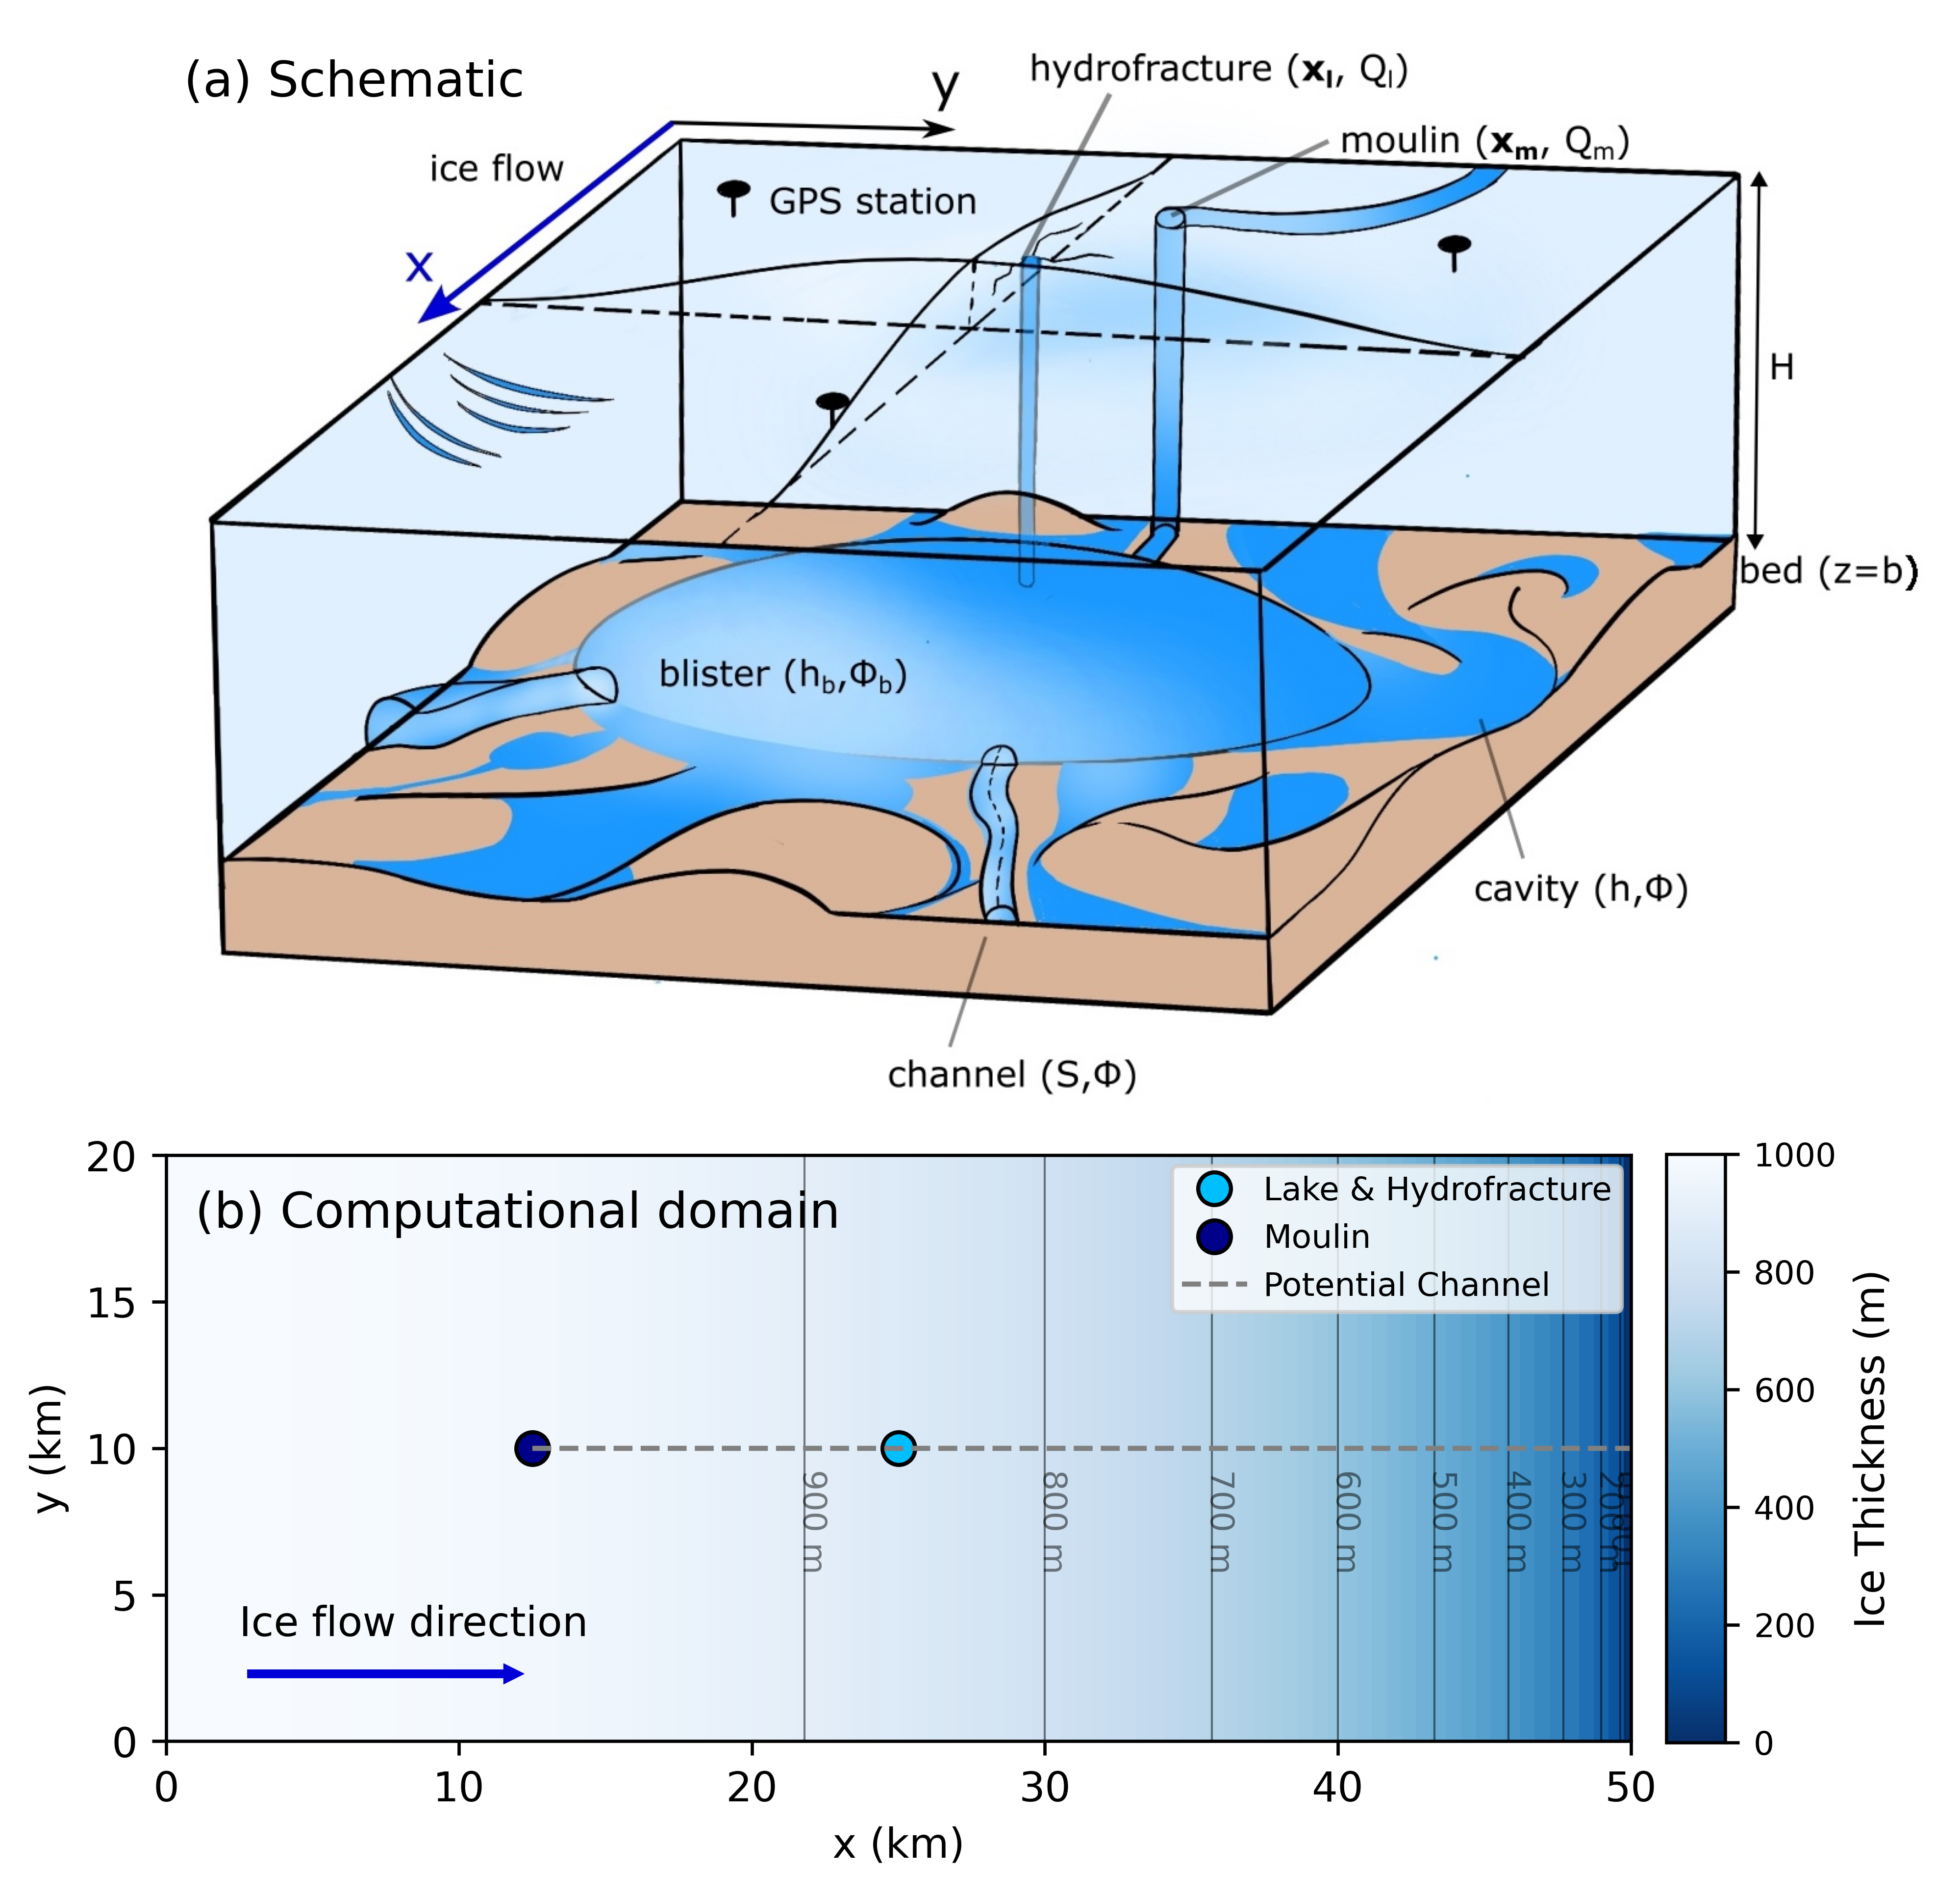
\includegraphics[width=0.8\linewidth]{./figures/Fig1_schematic.png}
    \caption{\textbf{Unified model set-up and computational domain.} (\textbf{a}) A schematic of the subglacial hydrology model including blister, cavity and channel components. (\textbf{b}) The computational domain for the reference cases.}
    \label{fig:schematic}
\end{figure}

\section{Results}\label{sec:results}
To illustrate our model set-up, we follow \citeA{hewitt2013Seasonal} to construct an idealised land-terminating ice sheet (Fig.~\ref{fig:schematic}b), with a length $L$ and a width $W$. The ice sheet sits on a flat bed with an elevation $b=0$. The ice thickness, denoted as $H$, is a function of along-flow coordinate $x$:
\begin{linenomath*}
\begin{equation}
    H = H_0\sqrt{1-\frac{x}{L}},\quad 0<x<L,
\end{equation}
\end{linenomath*}
where $H_0$ is a constant.

We are interested in how the blister propagates and leaks into the local drainage system. Meanwhile, we explore the seasonality of blister dynamics, specifically how blister propagation differs between summer and winter. For simplicity, we assume that there is one moulin with influx $Q_m$ at $\boldsymbol{x}_m=(0.25L,0.5W)$ and one downstream supraglacial lake at $\boldsymbol{x}_l=(0.5L,0.5W)$. The subglacial drainage system is initialised using two different moulin influxes $Q_m=0,10~\text{m}^3~\text{s}^{-1}$, which represent the wintertime and summertime surface runoff, respectively. After the drainage system reaches a steady state driven by $Q_m$, a lake-drainage input $Q_l$ is imposed at $\boldsymbol{x}_l$, delivering $V_l=10^{7}~\text{m}^3$ of water into the blister within $\sim3$ hr, after which $Q_l$ returns to zero. The drainage event triggers the formation and propagation of a blister and consequent evolution of the subglacial drainage system. Reference values for the physical variables used are given in \tabref{tab:parameters}.

\begin{table}[htbp]
    \centering
    \caption{Values of parameters used in the blister model.}
    \begin{tabular}{lcc}
        \hline
        Parameter & Symbol & Value \\   
        \hline
        Ice density & $\rho_i$ & $910~\text{kg}\cdot\text{m}^{-3}$ \\
        Water density & $\rho_w$ & $1000~\text{kg}\cdot\text{m}^{-3}$ \\
        Gravitational acceleration & $g$ & $9.81~\text{m}\cdot\text{s}^{-2}$ \\
        Ice thickness & $H_0$ & $1000~\text{m}$ \\
        Ice length & $L$ & $50~\text{km}$ \\
        Ice width & $W$ & $20~\text{km}$ \\
        Water viscosity & $\mu_{\text{eff}}$ & $10^{1}~\text{Pa}\cdot\text{s}$ \\
        Pre-wetted layer thickness & $h_0$ & $0.005~\text{m}$ \\
        Moulin influx & $Q_m$ & $0,10~\text{m}^3\cdot\text{s}^{-1}$ \\
        Lake drainage volume & $V_l$ & $10^{7}~\text{m}^3$ \\
        Lake drainage timescale & $\tau_l$ & $0.6~\text{hr}$ \\
        Young's modulus of ice & $E$ & $9.0\times10^{9}~\text{Pa}$ \\
        Poisson's ratio of ice & $\nu$ & $0.3$ \\
        Leakage coefficient & $\kappa$ & $10^{-10}$\\
        \hline    
    \end{tabular}
    \label{tab:parameters}
\end{table}

\subsection{Wintertime lake drainage}\label{sec:wintertime}
The wintertime subglacial drainage system is characterised by inefficient linked cavities. By spinning up the model without moulin input, the pre-blister drainage system only develops a thin cavity sheet due to melt sourced from constant geothermal heat fluxes. When the blister is generated by the lake drainage, it starts spreading roughly radially, and then propagates downstream along the ice-bed interface driven by the ice bending stress and gravity. \figref{fig:wintertime_drainage}a-d shows the magnitude of the water fluxes and the location of the blister margin, which we define as the $h_b=0.01$ m contour, at different times over this event. The water flux is defined as the sum of the fluxes in the cavity sheet, the channels and the blister. The $\phi$-contours of the cavity-channel system (\figref{fig:wintertime_drainage}a-d) indicate where the blister leaks into the surrounding drainage system and elevates the local hydraulic potential. However, since the cavity sheet is thin and channels are absent, the volume decrease of the blister is limited before the blister reaches the downstream, ice-margin boundary at $t\approx3$ d (\figref{fig:wintertime_drainage}e). The cavity sheet beneath the propagating blister is almost instantly saturated by leakage (i.e. the local cavity sheet is filled with water from the blister). Meanwhile, although the blister could contribute to channel growth \cite{dow2015Modeling}, this process is relatively slow compared with our simulation time of about 10 days. Therefore, the blister itself remains the main pathway for meltwater routing as it propagates downstream along the centerline.

The blister propagation causes surface uplift along its trajectory, which is captured by $h_b$ values at four hypothetical monitoring stations positioned downstream along the model centerline (\figref{fig:wintertime_drainage}f). The normalised blister volume and the normalised distance from the lake to the blister front are also presented in \figref{fig:wintertime_drainage}f. The average front velocity is approximately $0.1~\text{m}~\text{s}^{-1}$, which is close to the lower end of subglacial flood propagation speed observations summarised in \citeA{stevens2022Tidewaterglacier}. A detailed exploration of the blister velocity and geometry controlled by the parameter space is presented in \secref{sec:discussion}.

\begin{figure}[!ht]
    \centering
    
\includegraphics[width=0.85\linewidth]{./figures/Fig2_wintertime.png}
    \caption{ \textbf{Full water fluxes and blister profiles for a wintertime lake-drainage event.} \textbf{(a)} Pre-drainage water flux and positions of the moulin, lake, and hypothetical monitoring stations (S1-S3), marked with coloured dots or triangles. \textbf{(b)}-\textbf{(d)} Water flux magnitude (background colour and colorbar) and $0.01$-m contour (blue line) of the blister thickness at $t=0.0$ d, $t=1.0$ d and $t=10.0$ d. Black lines are contours of the hydraulic potential $\phi$. \textbf{(e)} Time series of the fluxes. The blue line is the lake-drainage input (moulin input is zero in this case). The green line is the net outflux from the right boundary. The orange line is the leakage from the blister to the drainage system. \textbf{(f)} Time series of the blister thickness at different locations along the centerline. The dashed-grey line is the ratio of the blister volume to the volume of the drained lake ($V_b/V_l$). The solid-grey line is the ratio of the distance from the lake position to the blister front, to the total distance from the lake to the downstream boundary. When the blister front reaches the downstream boundary, this ratio equals 1.}
    \label{fig:wintertime_drainage}
\end{figure}

\subsection{Summertime lake drainage}\label{sec:summertime}
In contrast to wintertime drainage events, summertime blisters enter an evolving cavity-channel system and could rapidly leak into an efficient channel network. For a summertime case, we use the same computational domain and parameter values (\figref{fig:wintertime_drainage}b) and spin up the model with a moulin input of $Q_m=10~\text{m}^3~\text{s}^{-1}$ (\figref{fig:summertime_drainage}a). This leads to the formation of a channel with a cross section of approximately $10~\text{m}^2$ along the ice centreline. Once the blister forms, the channel transports the blister water out of the domain quickly, and the perturbation caused by the lake drainage propagates through the channel almost instantaneously (\figref{fig:summertime_drainage}e); the pressure perturbation caused by the blister is small in the vicinity of the channel (\figref{fig:summertime_drainage}b-d). Therefore, the blister decays rapidly in volume (\figref{fig:summertime_drainage}f), starts vanishing from the centreline (i.e., where the channel is located), and then finally leaves two small-thickness branches on both sides of the channel (\figref{fig:summertime_drainage}d). 

\begin{figure}[!ht]
    \centering
    
\includegraphics[width=0.85\linewidth]{./figures/Fig3_summertime.png}
    \caption{\textbf{Evolution of the subglacial drainage system and blister following a summertime lake drainage event.} Figure convention is the same as \figref{fig:wintertime_drainage}, except that the moulin influx, represented by the red line in (\textbf{e}), is non-zero, which leads to a subglacial channel along the centerline. The blister leaks into the drainage system more quickly.}
    \label{fig:summertime_drainage}
\end{figure}

Meanwhile, as the perturbation caused by the lake drainage propagates rapidly through the channel network, the blister may pressurise the channel, leading to a transient increase in water pressure further upstream at the moulin location. If this pressure increase causes the effective pressure at the moulin location to reduce below zero, the moulin input can be redirected away from the cavity-channel system (\eqnref{eq:mass_conservation_blister}), triggering the formation of a secondary blister (this does not occur in Figure 3, but has been observed in other test cases).  Consequently, blister dynamics during summer can be more complicated than in winter, and strongly influenced by interactions between blister propagation and the prevailing channel network.

\section{Discussion}\label{sec:discussion}
The unified blister and subglacial hydrology model extends existing subglacial hydrology models by capturing transient responses to rapid lake drainage events. Previous studies, such as the one-dimensional coupling of an elastic blister and subglacial drainage system by \citeA{pimentel2010Numerical}, and the combination of an idealised hydrofracture blister model with one-dimensional subglacial hydrology models by \citeA{rice2015Time} and \citeA{dow2015Modeling}, did not account for sideways spreading or realistic downslope blister propagation. In contrast, our two-dimensional framework allows the blister to spread laterally and propagate downslope over realistic topography, enabling testable predictions of blister geometry and propagation velocity.

Our results for an idealised, land-terminating ice sheet suggest a trade-off between blister propagation and leakage into the surrounding subglacial drainage system. This trade-off controls the speed and spatial extent of surface velocity and ice uplift waves observed following supraglacial lake drainage events \citeg{maier2023Wintertime}. In this section, we examine how blister propagation velocity depends on effective viscosity $\mu_{\text{eff}}$ and lake drainage volume $V_l$ under conditions of negligible leakage, and subsequently investigate how leakage rate is controlled by the coefficient $\kappa$ in our ad-hoc leakage lengthscale formulation ($l=\kappa h_b$) under conditions of slow blister propagation (with a velocity of about $5\times10^{-4}~\text{m}~\text{s}^{-1}$). Results are then compared with previously observed lake drainage events.

\subsection{Propagation velocity}\label{sec:propagation}
Given that propagation velocity is a common observable of subglacial floods, it is important to understand the controls on propagation velocity in our model, and to examine the model's ability to propagate blisters at realistic velocities. Our two reference cases of blister propagation have front velocities of approximately $0.1~\text{m}~\text{s}^{-1}$ (\figref{fig:wintertime_drainage}, \figref{fig:summertime_drainage}). However, velocity waves caused by rapid lake drainage events can propagate with a speed up to $1.0~\text{m}~\text{s}^{-1}$ \citeg{bjornsson2003Subglacial}. \citeA{stevens2022Tidewaterglacier} summarised a range of flood propagation speeds following, not only lake drainages, but also other types of subglacial floods such as jökulhlaups and precipitation events; they found that the propagation velocity can vary widely, from $10^{-2}~\text{m}~\text{s}^{-1}$ to $1.0~\text{m}~\text{s}^{-1}$, depending on the flood type and the local subglacial drainage system. 

Here we explore how the propagation velocity in our model depends on the effective viscosity $\mu_{\text{eff}}$ and the lake drainage volume $V_l$ under the assumption of negligible leakage (i.e., $\kappa=0$). (\secref{sec:regional_study} later considers the effects of leakage on propagation in a realistic setting.) The effective viscosity $\mu_{\text{eff}}$ accounts for turbulence, ice-bed toughness and other characteristics of the ice-bed interface that contribute to energy loss during propagation. Effective viscosity can have a more complex formulation \cite{zimmerman2004non,sommers2018SHAKTI,hill2024Improved}, but here we treat the parameter as a constant for simplicity. We define the front as the downstream end of the blister where the blister thickness exceeds a threshold of $10^{-2}~\text{m}$. The propagation velocity $\bar{v}$ is then defined as the average speed of the downstream ($x$-direction) front during the propagation.

We vary $\mu_{\text{eff}}$ from $10^{-3}~\text{Pa}~\text{s}$ to $10^{3}~\text{Pa}~\text{s}$, covering a wide range of possible values. The lake drainage volume $V_l$ is varied from $10^{6}~\text{m}^3$ to $10^{8}~\text{m}^3$, which covers the typical range of supraglacial lake volumes in Greenland \citeg{melling2024Evaluation}. For a fixed $V_l$, the propagation velocity $\bar{v}$ decreases with increasing $\mu_{\text{eff}}$, and undergoes a transition from a bending-dominated regime to a gravity-dominated regime (\figref{fig:blister_velocity}a). For $\mu_{\text{eff}}=10^{-3}~\text{Pa}~\text{s}$, $\bar{v}\sim \mu_{\text{eff}}^{-1/11}$, consistent with previous results for a bending-dominated regime \cite{peng2020Viscous}(See \appref{apdx:scalings} for details). As $\mu_{\text{eff}}$ increases, the dependence transitions to $\bar{v}\sim \mu_{\text{eff}}^{-1}$ where the downslope gravity takes control, consistent with the scaling in \citeA{tobin2023Evolution}. By comparing the numerical results with the observed range of the propagation velocity, we can infer that the effective viscosity $\mu_{\text{eff}}$ likely lies between $10^{-2}~\text{Pa}~\text{s}$ and $10^{3}~\text{Pa}~\text{s}$ for typical lake drainage events with $V_l$ between $10^{6}~\text{m}^3$ and $10^{8}~\text{m}^3$, indicating that the effective viscosity is much larger than the viscosity of water ($10^{-3}~\text{Pa}~\text{s}$).

\begin{figure}[!ht]
    \centering
    
\includegraphics[width=1.0\linewidth]{./figures/Fig5_velocity.png}
    \caption{\textbf{Propagation velocity of the blister front as a function of effective viscosity $\mu_{\text{eff}}$ and lake drainage volume $V_l$.} (\textbf{a}) The propagation velocity $\bar{v}$ as a function of $\mu_{\text{eff}}$ for different lake drainage volumes $V_l$. The dashed line is the scaling in the bending-dominated regime ($\bar{v}\sim \mu_{\text{eff}}^{-1/11}$), while the dash-dotted line is the gravity-dominated regime ($\bar{v}\sim \mu_{\text{eff}}^{-1}$). Note these lines just represent the trend of the dependence, and the prefactors vary among different cases and are not included. (\textbf{b}) The propagation velocity $\bar{v}$ as a function of $V_l$ for different effective viscosities $\mu_{\text{eff}}$. The dashed line and the dash-dotted line are the scalings in the bending-dominated regime ($\bar{v}\sim V_l^{5/22}$) and the gravity-dominated regime ($\bar{v}\sim V_l^{5/4}$), respectively.}
    \label{fig:blister_velocity}
\end{figure}

Another key factor influencing $\bar{v}$ is the blister volume. During winter, blister volume closely matches the lake drainage input volume $V_l$ as the leakage is negligible. As shown in \figref{fig:blister_velocity}b, the lake volume has a clear control on $\bar{v}$: for typical lake drainage events with $V_l$ lying between $10^{6}~\text{m}^3$ and $10^{8}~\text{m}^3$, the velocity ranges from $10^{-3}~\text{m}~\text{s}^{-1}$ (i.e., nearly a fixed-position blister) to $10^{1}~\text{m}~\text{s}^{-1}$ (i.e., much faster than observed). For sufficiently small $\mu_{\text{eff}}$, the velocity follows a bending-dominated regime with $\bar{v}\sim V_l^{5/22}$ regardless of $V_l$. As $\mu_{\text{eff}}$ increases, the dependence transitions to a gravity-dominated regime with $\bar{v}\sim V_l^{5/4}$. 

By varying both $\mu_{\text{eff}}$ and $V_l$, our model can reproduce a wide range of blister propagation velocities that are consistent with observed subglacial flood propagation speeds. This suggests that our model effectively captures the essential physics governing blister propagation following supraglacial lake drainage events.

\subsection{Leakage}
In \secref{sec:propagation}, we explored blister propagation under the assumption of negligible leakage ($\kappa=0$). However, in reality, blister leakage into the surrounding drainage system can be significant, especially during summertime drainage events when an efficient channel network exists. Here we explore how the leakage rate depends on the leakage coefficient $\kappa$ in our ad-hoc formulation of the leakage lengthscale $l=\kappa h_b$. We consider two scenarios: a wintertime drainage event with no background moulin input ($Q_m=0$), and a summertime drainage event with a background moulin input of $Q_m=10~\text{m}^3~\text{s}^{-1}$, which leads to channel formation along the ice centreline. The effective viscosity is set to $\mu_{\text{eff}}=10^3~\text{Pa}~\text{s}$, causing the blister to move slowly and preventing it from reaching the downstream boundary during the simulation period. We vary $\kappa$ to explore its influence on the leakage behaviour.

The time series of the normalised blister volume $V_b/V_l$ for different values of $\kappa$ are shown in \figref{fig:leakage}a. The volume decreases more rapidly with increasing $\kappa$, indicating a higher leakage rate. For the same $\kappa$, the summer case exhibits a higher leakage rate compared to the winter case, due to the presence of an efficient channel that quickly transports water away. However, the volume decay follows neither a simple power-law \citeg{tobin2023Evolution} nor an exponential form \citeg{lai2021Hydraulic}. Here, we focus on the overall leakage rate rather than the detailed temporal evolution. To quantify this rate, we calculate the time-averaged volume-loss rate over the period from $t=0$ to $t=30$ d, during which the blister hardly moves. In both summer and winter cases, the volume-loss rate magnitude increases linearly with $\kappa$ at small values of $\kappa$, and begins to deviate from the linear trend as $\kappa$ increases (\figref{fig:leakage}b). This transition occurs when leakage reaches the capacity of the surrounding drainage system; that is, the leakage rate is limited by the ability of the cavity-channel system to transport water away, rather than the leakage process itself.

\begin{figure}[!ht]
    \centering
    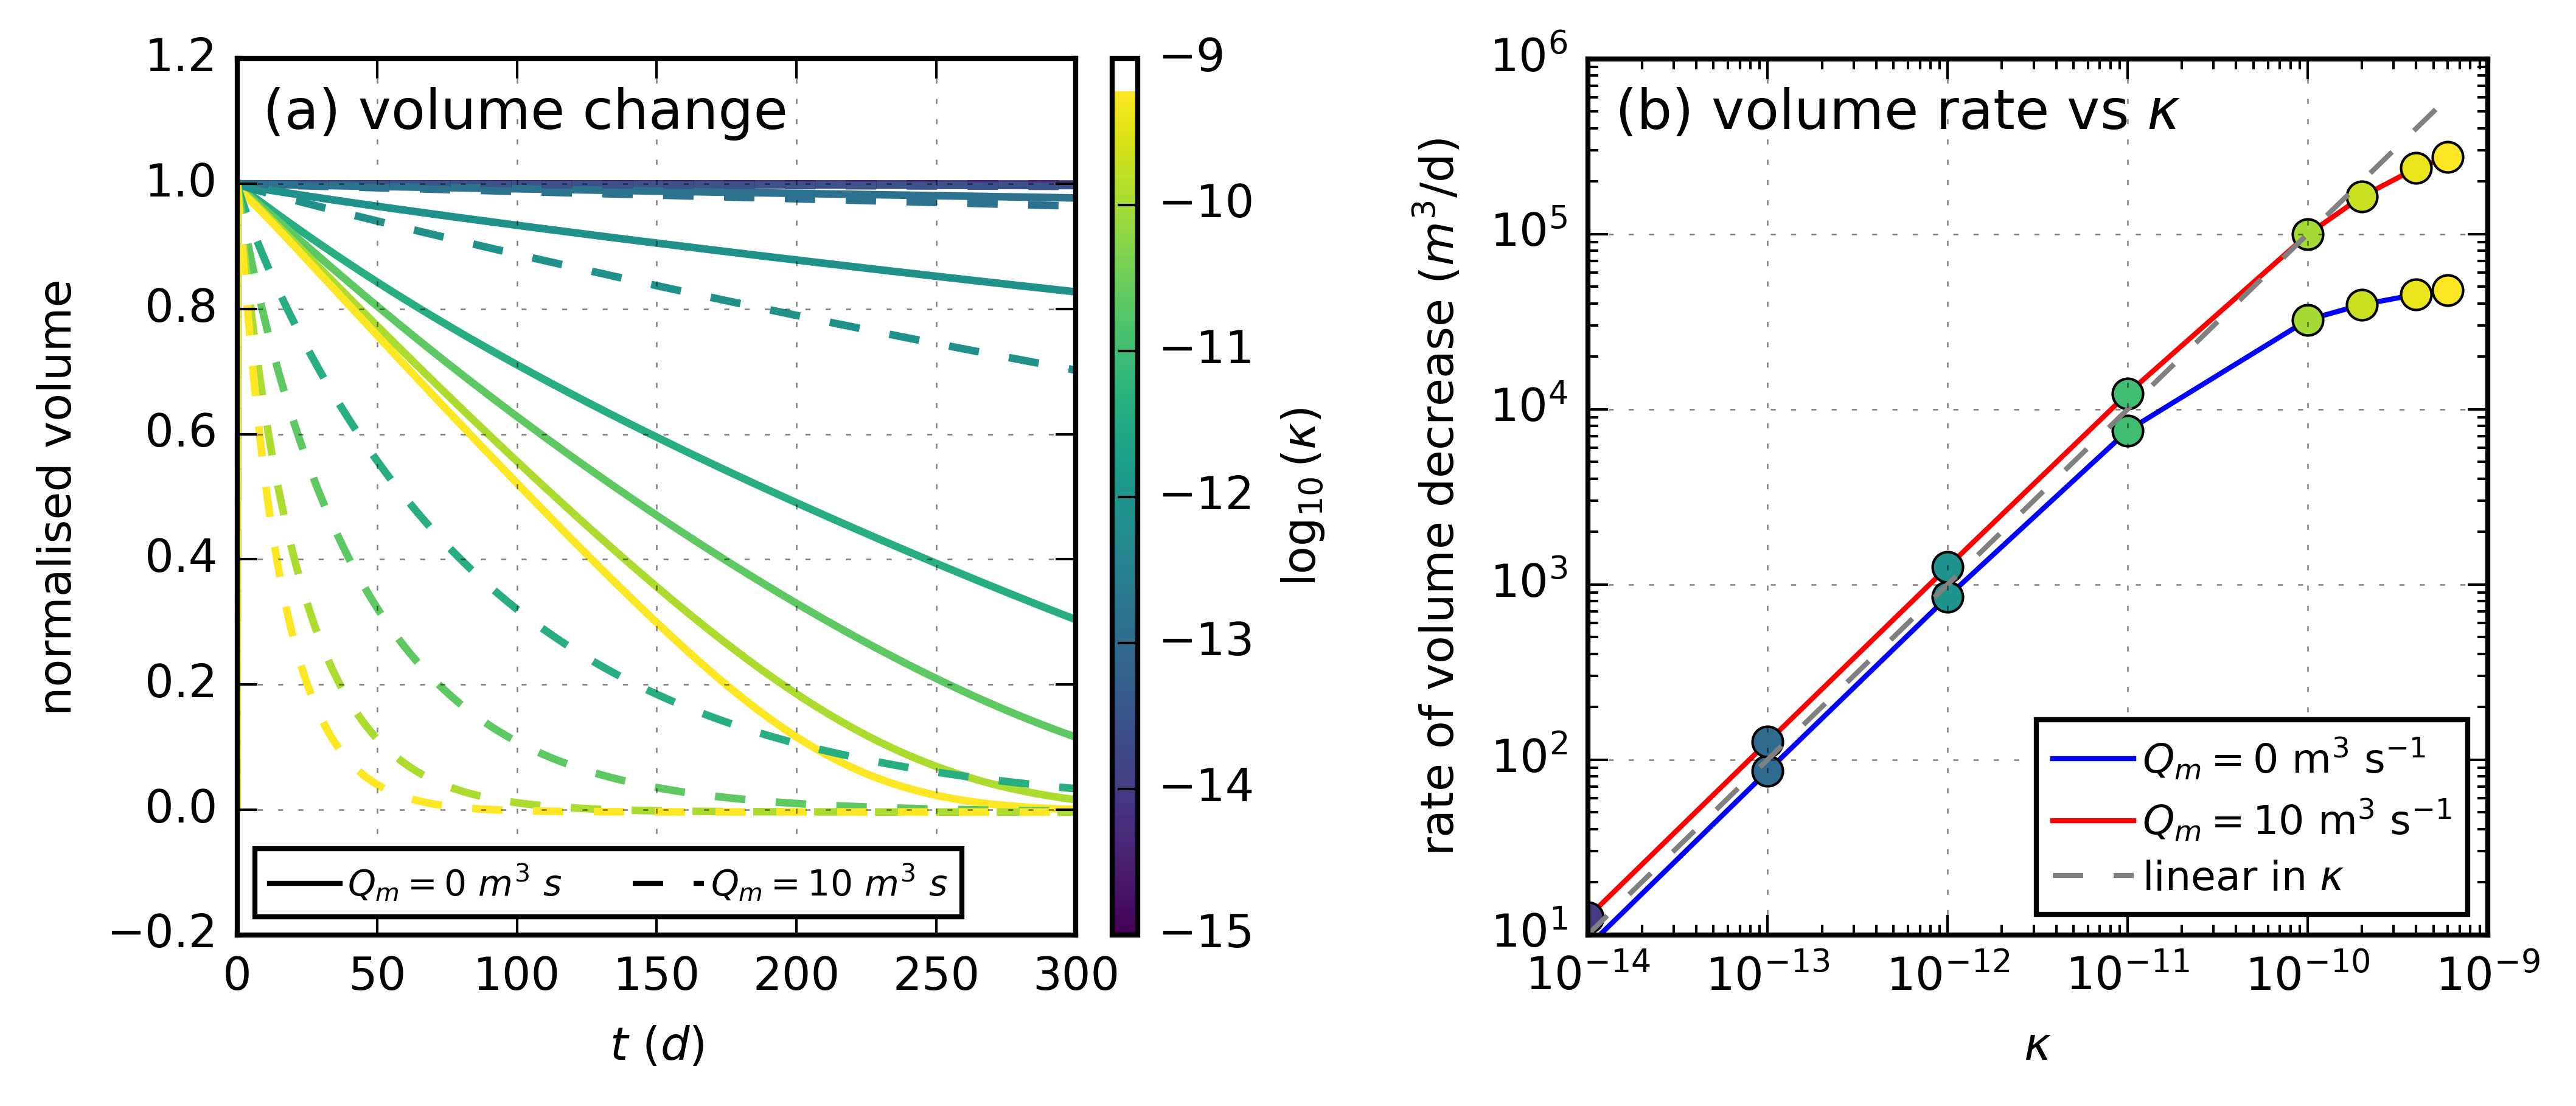
\includegraphics[width=1.0\linewidth]{./figures/Fig6_volume.png}
    \caption{\textbf{Wintertime and summertime blister volume loss with different values of $\kappa$}. (\textbf{a}) Time series of the normalised blister volume $V_b/V_{l}$ due to leakage for different values of $\kappa$ in the winter case (solid lines) and the summer case (dashed lines). (\textbf{b}) The magnitude of the time-averaged volume loss rate from $t=0$ to $t=30$ d as a function of $\kappa$ for the winter case (blue) and the summer case (red). The dashed line is a linear reference. Colours correspond to different values of $\kappa$ in (\textbf{a}).}
    \label{fig:leakage}
\end{figure}

\section{A regional study in western Greenland}\label{sec:regional_study}
To demonstrate the applicability of our model to an observed lake drainage event, we simulate an idealised scenario that mimics the wintertime lake drainage cascades documented by \citeA{maier2023Wintertime} across a land-terminating ice-sheet region in western Greenland. During the event in March 2018, a total of 18 supraglacial lakes drained sequentially, delivering approximately $1.8\times10^{8}~\text{m}^3$ of water to the ice-sheet bed. Three-component interferometric surface velocity fields and decomposition modelling indicate that the resulting subglacial flood propagated approximately $160$ km over a period of about $30$ days, causing ice-flow acceleration along the flood pathway \cite{maier2023Wintertime}. To replicate this event, we use a $140~\text{km}\times80~\text{km}$ model domain covering the same region studied by \citeA{maier2023Wintertime}. Following \citeA{stevens2018Relationship}, the bed topography and ice surface elevation are extracted from IceBridge BedMachine Greenland Version 2 \cite{morlighem2014Deeply} and the Greenland Ice Mapping Project (GIMP) digital elevation model \cite{howat2014Greenland}, respectively. Ice thickness is calculated as the difference between ice surface elevation and bed elevation. The model domain and bed topography are shown in \figref{fig:regional_study}a.

We assume zero moulin input ($Q_m=0$) for the wintertime drainage conditions. The model is spun up for $5$ years to allow the cavity-channel system to reach a steady state driven by basal melt from constant geothermal heat fluxes and basal frictional heating. Due to the regularisation parameter $h_0=0.005~\text{m}$ in \eqnref{eq:mass_conservation_blister}, the blister layer $h_b$, initially set to zero, develops small, but non-zero, thickness during the spin-up period due to hydraulic potential gradients resulting from ice overburden and bed topography. This results in minor water redistribution within the blister layer even prior to lake drainage. However, the blister thickness remains sufficiently small to have negligible influence on the cavity-channel system and subsequent subglacial flood dynamics following lake drainage. A more physically consistent regularisation scheme, such as incorporating fracture mechanics \cite{lister2019Viscous}, could resolve this issue, but this is left to future work.

Additionally, we idealise the lake drainage event as a single-point input at $(x,y)=(40~\text{km},-20~\text{km})$, delivering a total water volume of $1.8\times10^{8}~\text{m}^3$ over a timescale of $\tau_l=0.6$ hr. We first demonstrate the model behaviour by considering a case with no leakage ($\kappa=0$). Therefore, the blister remains the only pathway for meltwater routing and is decoupled from the cavity-channel system, which evolves independently only due to melt sourced from basal frictional and geothermal heat. The effective viscosity is set to $\mu_{\text{eff}}=20~\text{Pa}~\text{s}$, ensuring the modelled propagation velocity is consistent with the observed value \cite{maier2023Wintertime}.

On realistic topography, the blister does not propagate along a straight line as in the idealised cases in \secref{sec:results}. Instead, it propagates toward the ice margin following a tortuous path determined by a combination of ice overburden, bed topography, and ice bending stress. In \figref{fig:regional_study}a-d, we present both the blister water flux magnitude and the blister $0.1$-m thickness contour at various times. The blister reaches the ice margin in $30$ days (\figref{fig:regional_study}d-e), corresponding to an average propagation velocity of approximately $0.1~\text{m}~\text{s}^{-1}$. The $h_b$ time series at the lake location and three downstream, hypothetical monitoring stations show diverse patterns of surface uplift (\figref{fig:regional_study}f). When the drainage occurs, the lake location and station S1 both experience an uplift over $1$ m, which subsequently decays. Other downstream locations experience smaller uplifts with relatively slower decay rates. Notably, due to the presence of the blister's tail region, uplift at these downstream locations persists long after the blister front has passed, which could help explain the prolonged uplift signals observed after lake drainage events by \citeA{doyle2013Ice} and \citeA{mejia2021Isolated}. Therefore, caution should be exercised when interpreting surface-uplift durations, as these signals may not directly reflect the timing of blister-front passage.

\begin{figure}[!ht]
    \centering
    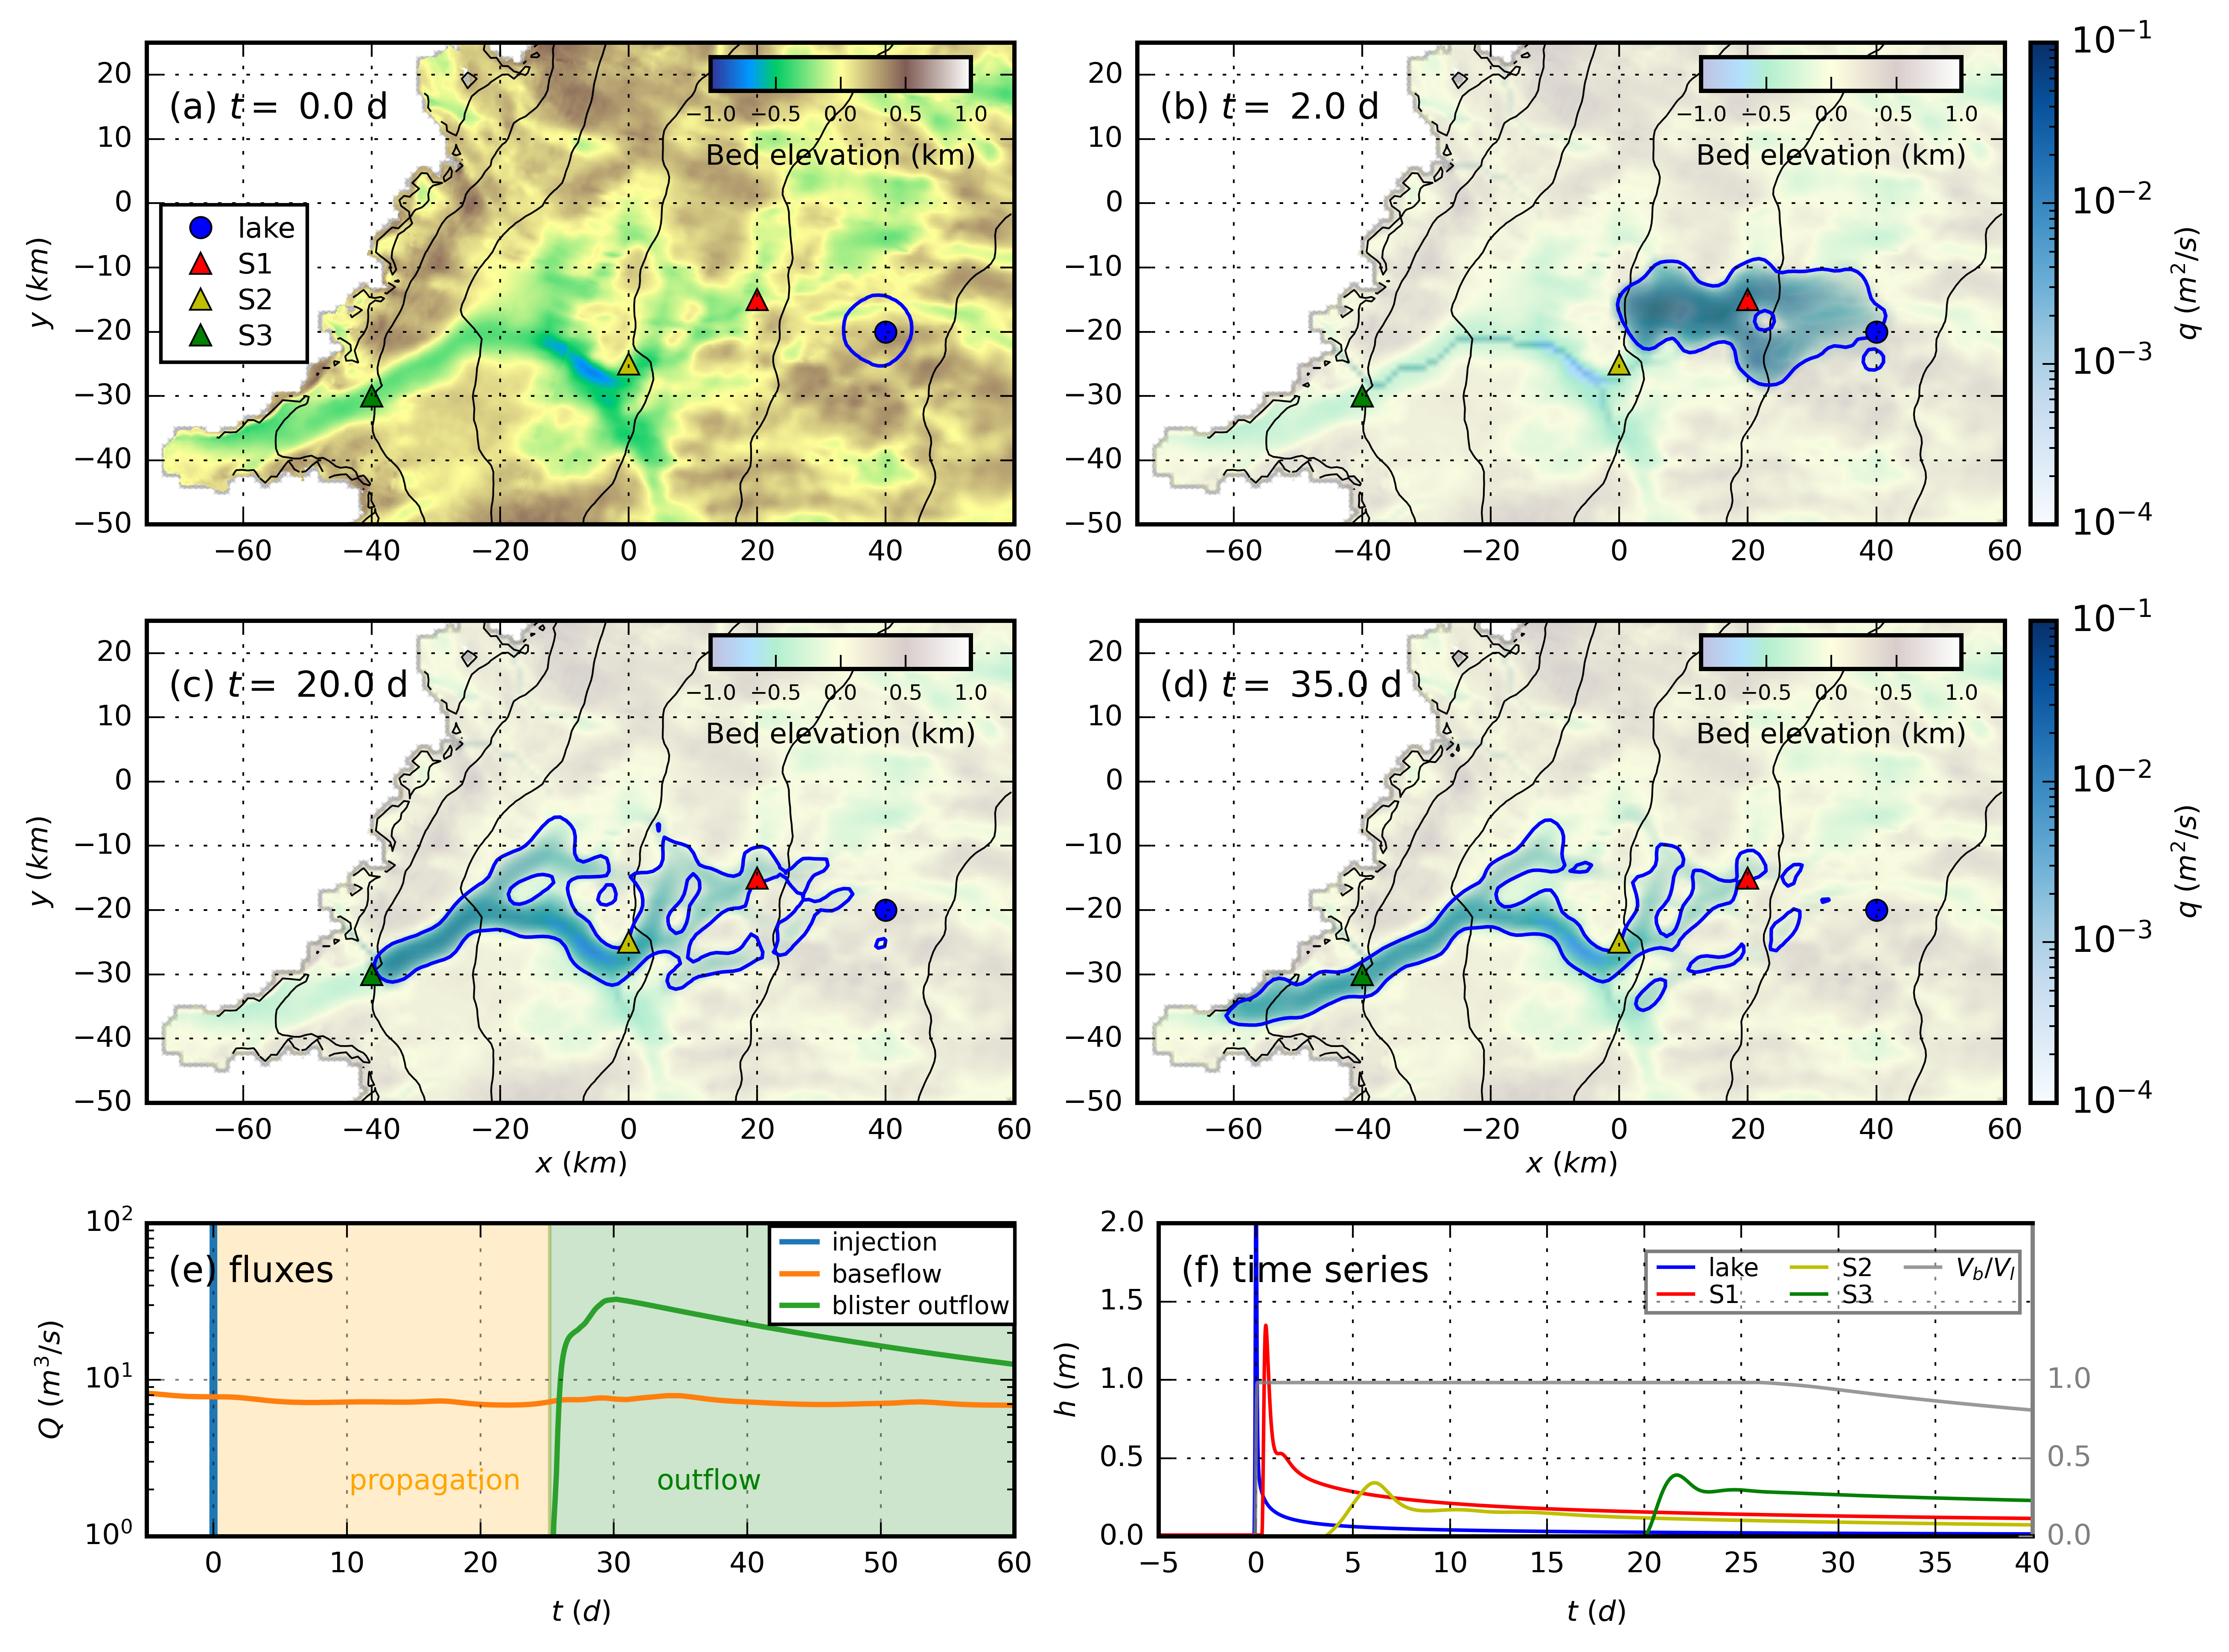
\includegraphics[width=1.0\linewidth]{./figures/Fig7_regional.png}
    \caption{\textbf{Simulation of a wintertime lake drainage event in western Greenland, with $\mu_{\text{eff}}=20~\text{Pa}~\text{s}$ and $\kappa=0$.} (\textbf{a}) Bed topography and positions of the lake and hypothetical monitoring stations (S1-S3), marked with coloured dots and triangles. (\textbf{b})-(\textbf{d}) Water flux magnitude (background blue colour) and $0.1$-m contour (blue line) of the blister thickness at $t=2.0$ d, $t=20.0$ d and $t=35.0$ d. Black lines are contours of the hydraulic potential $\phi$. (\textbf{e}) Time series of the fluxes. The blue line is the lake input, with maximum $Q_{l}\sim3000~\text{m}^3~\text{s}^{-1}$. The orange line is the background water outflow of the cavity-channel system. The green line is the blister outflow. (\textbf{f}) Time series of the blister thickness at different locations along the blister path. The grey line is the ratio of the blister volume to the volume of the drained lake ($V_b/V_l$).}
    \label{fig:regional_study}
\end{figure}

However, our assumption of no leakage is likely unrealistic since observed uplifts and velocity anomalies following lake drainage events typically last only a few days to weeks \citeg{maier2023Wintertime,stevens2022Tidewaterglacier,mejia2021Isolated, doyle2013Ice}. Therefore, blister leakage could be as critical as propagation in determining subglacial meltwater routing and surface uplift patterns. To explore the effects of leakage, we conduct a series of simulations using $\mu_{\text{eff}}=10~\text{Pa}~\text{s}$ and various values of $\kappa$, with results summarised in \figref{fig:regional_study_time_series}. For simplicity, we define the blister front position as the westernmost point of the blister where its thickness exceeds $0.1$ m. As indicated by \eqnref{eq:leakage}, the blister volume decreases more rapidly with increasing $\kappa$ (\figref{fig:regional_study_time_series}a). In \figref{fig:regional_study_time_series}b, we plot the distance from the lake to the blister front, $L_b$, as a function of time. As leakage increases (i.e., with larger $\kappa$), the blister front propagates more slowly due to rapid volume loss, and propagation may eventually halt before reaching the ice margin if $\kappa$ becomes sufficiently large. The drained water is then primarily routed through the channel network. In the supplementary material, we provide videos illustrating the blister propagation and leakage for different values of $\kappa$.

By combining observed propagation speeds, surface uplift patterns, and water outflow locations and timings at the ice margin, this model can potentially constrain the values of $\mu_{\text{eff}}$ and $\kappa$ for specific lake drainage events, thereby determining the primary pathways of subglacial flood routing. 

\begin{figure}[!ht]
    \centering
    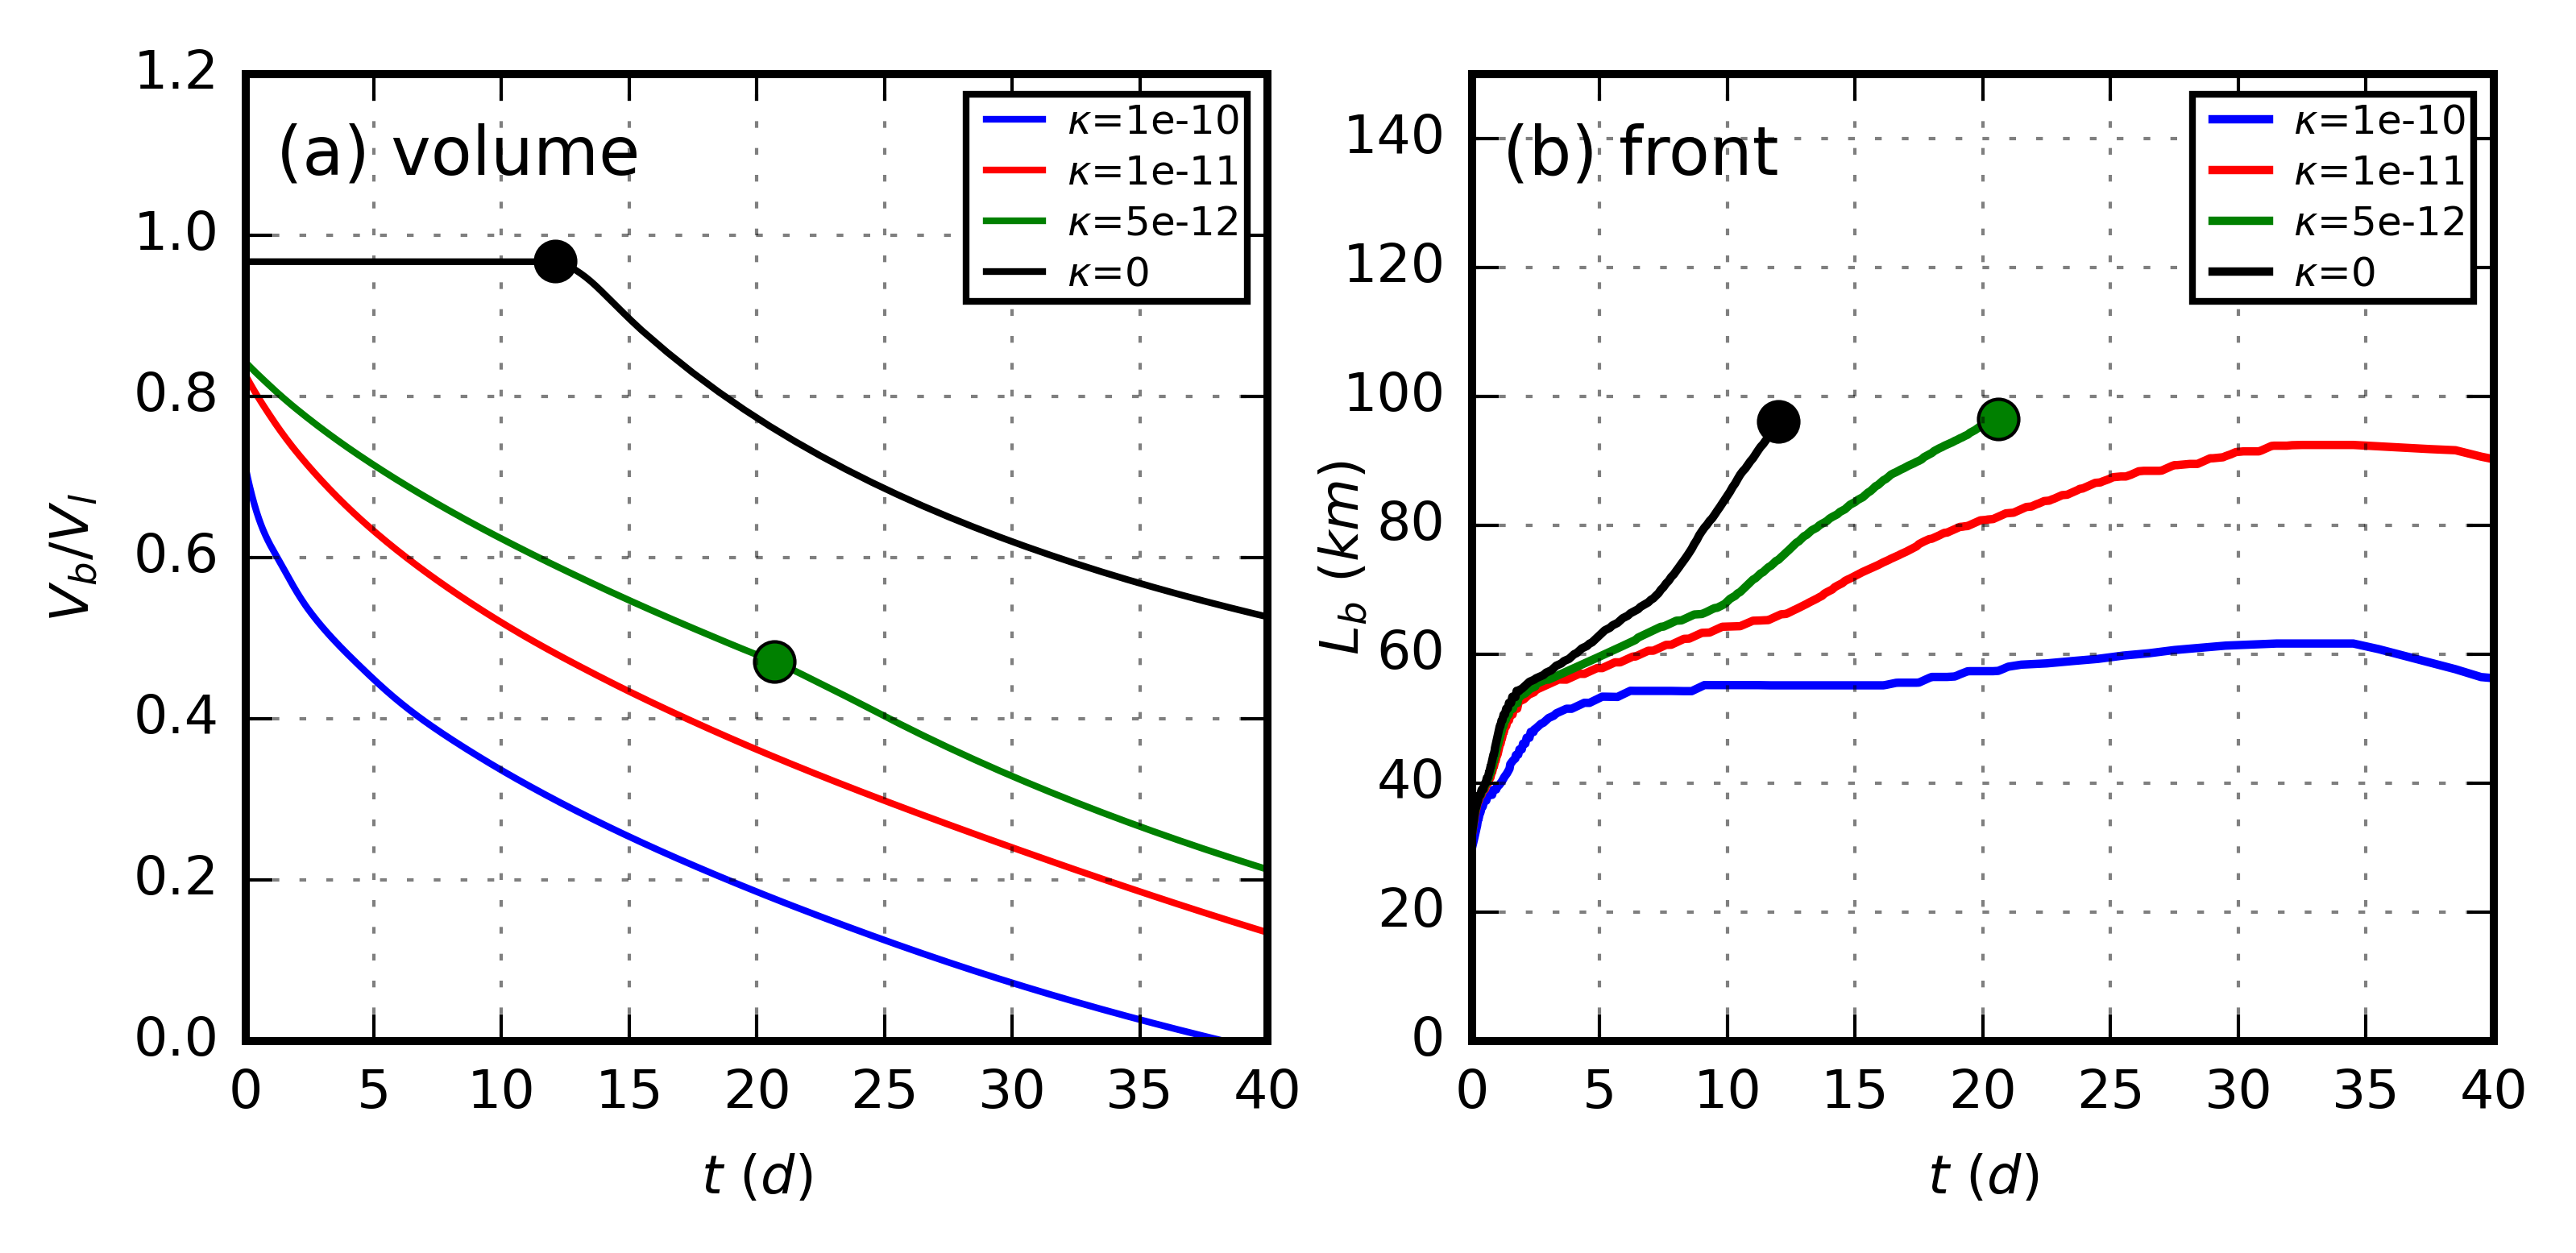
\includegraphics[width=1.0\linewidth]{./figures/Fig8_regional_front_volume.png}
    \caption{\textbf{Time series of the blister volume and front position in the regional study with different values of $\kappa$.} (\textbf{a}) Time series of the normalised blister volume $V_b/V_{l}$, and (\textbf{b}) distance from the lake to the blister front $L_b$, for different values of $\kappa$ with $\mu_{\text{eff}}=10~\text{Pa}~\text{s}$. Dots indicate the time when the blister front reaches the ice margin, with colours representing different values of $\kappa$. No dots are shown for cases where the blister front does not reach the ice margin.}
    \label{fig:regional_study_time_series}
\end{figure}

\section{Conclusion}\label{sec:conclusion}
In this study, we have developed a unified model that couples blister dynamics with the subglacial drainage system, allowing us to explore the transient effects of rapid supraglacial lake drainage events. Our model captures the seasonal variability of blister dynamics, demonstrating that summertime drainage leads to efficient blister leakage into existing channel networks, while wintertime drainage results in persistent blisters that act as primary pathways for meltwater transport. The dynamics of blister propagation and leakage are governed by effective viscosity and a characteristic leakage length scale. An exploration of the parameter space reveals that blister propagation velocity can vary significantly, depending on the effective viscosity and the volume of the lake drainage input.

This integrated model enables us to investigate blister dynamics and how blister formation and propagation interact with, and modify, subglacial hydrology under realistic ice-sheet conditions. Our regional simulation of a wintertime lake drainage event in western Greenland produces results consistent with observed propagation speeds and subglacial flood extents. The model can facilitate the interpretation of observed surface uplift and ice-velocity anomalies following supraglacial lake drainage events. Future work will focus on developing consistent formulations of effective viscosity and leakage, and coupling the current model to an ice-sheet sliding model to better capture feedbacks between ice dynamics and subglacial hydrology.

\appendix
\section{Model equations for the cavity-channel system}\label{apdx:subglacial_hydrology}
The subglacial hydrology model used in this study is based on the two-component model by \citeA{hewitt2013Seasonal}, which consists of a cavity sheet and channels. We solve for the cavity sheet thickness $h$, the channel cross sections $S$, and the hydraulic potential $\phi$ using the mass conservation equation given by
\begin{linenomath*}
\begin{equation}\label{eq:mass_conservation_cavity}
    \pdiff{h}{t} + \nabla \cdot \boldsymbol{q} + \pdiff{S}{t} \delta(\boldsymbol{x}_c) +\pdiff{Q}{s} \delta(\boldsymbol{x}_c) = m + M \delta(\boldsymbol{x}_c) + \sum_{m}Q_m\delta\left(\boldsymbol{x}_m\right)\mathcal{H}\left(N(\boldsymbol{x}_m)\right) + Q_b,
\end{equation}
\end{linenomath*}
where $\boldsymbol{q}$ is the flux of the cavity sheet, $\boldsymbol{x}_c$ is the position of channels, $Q$ is the channel flux,  $s$ is an along-channel coordinate, $\delta(\boldsymbol{x}_c)$ is the delta function at the channels. The right hand side includes the source terms: $m$ is the cavity melting rate due to geothermal heat flux and friction, $M$ is the channel melting rate, $Q_m$ is the input from moulins, and $Q_b$ is the leakage from the blister. For simplicity, the cavity flux $\boldsymbol{q}$ is treated using a Darcy-like parameterisation, such that
\begin{linenomath*}
\begin{equation}
    \boldsymbol{q}=-K_s h^{3}\Grad\phi,
\end{equation}
\end{linenomath*}
where $K_s$ is a permeability constant. The hydraulic potential $\phi$ is expressed as
\begin{linenomath*}
\begin{equation}
    \phi = \rho_w g b + p_w,
\end{equation}
\end{linenomath*}
where $\rho_w$ is the density of water, $g$ is gravitational acceleration, $b$ denotes bed elevation, and $p_w$ is the subglacial water pressure. The water pressure $p_w$ is expressed in terms of the effective pressure $N$, given by the difference between the ice overburden pressure and the subglacial water pressure:
\begin{linenomath*}
\begin{equation}
    N = \rho_i g H - p_w,
\end{equation}
\end{linenomath*}
where $\rho_i$ is the density of ice and $H$ is the ice thickness.

The cavity sheet evolves according to the balance between opening due to sliding and melting, and closing due to viscous creep:
\begin{linenomath*}
\begin{equation}
    \pdiff{h}{t} = \frac{\rho_w}{\rho_i}m + U_b\left(h_r-h\right)/l_r - \frac{2 A}{n^n}h|N|^{n-1}N,
\end{equation}
\end{linenomath*}
where $m$ is the cavity melting rate, $U_b$ is the sliding velocity, $h_r$ is the reference thickness, $l_r$ is the reference length scale, $A$ and $n$ are the Glen's flow law parameters. Since this study does not incorporate a coupled ice-sheet model, the basal sliding velocity $U_b$ is assumed to be constant. Additionally, the cavity melting rate $m$ is set to a constant value given by $\frac{G}{\rho_w L}$, where $G$ represents the geothermal heat flux and $L$ denotes the latent heat of fusion.

The channel flux $Q$ is formulated using a turbulent flow parameterisation
\begin{linenomath*}
\begin{equation}
    Q = -K_c S^{5/4}\left|\pdiff{\phi}{s}\right|^{-1/2}\pdiff{\phi}{s},
\end{equation}
\end{linenomath*}
where $K_c$ is a constant. The channel cross section $S$ evolves according to the balance between melting opening and viscous creep closure:
\begin{linenomath*}
\begin{equation}
    \pdiff{S}{t} = \frac{\rho_w}{\rho_i}M - \frac{2 A}{n^n}S|N|^{n-1}N,
\end{equation}
\end{linenomath*}
where $M$ is the melting rate of the channel, parameterised as
\begin{linenomath*}
\begin{equation}\label{eq:channel_melting}
    M = \frac{\left|Q \partial\phi/\partial s\right| + \lambda_c\left|\boldsymbol{q}\cdot\Grad\phi\right|}{\rho_w L}.
\end{equation}
\end{linenomath*}
Here, $\lambda_c$ is the ``incipient channel width" \cite{hewitt2013Seasonal} that accounts for the lengthscale over which the channel can capture melt from the surrounding cavity sheet. In \tabref{tab:hydrology_parameters}, we summarise the parameters relevant to the cavity-channel system used in both the reference cases (\secref{sec:results}) and the regional study (\secref{sec:regional_study}).
\begin{table}[htbp]
    \centering
    \caption{\textbf{Values of parameters of the subglacial hydrology model in the reference cases in \secref{sec:results}.} Values in parentheses are used in the regional studies in \secref{sec:regional_study} if different from the reference cases.}
    \begin{tabular}{lcc}
        \hline
        Parameter & Symbol & Value \\   
        \hline
        Latent heat of melting & $L$ & $3.35\times10^{5}~\text{J}\cdot\text{kg}^{-1}$ \\
        Specific heat capacity of water & $c$ & $4.2\times10^{3}~\text{J}\cdot\text{kg}^{-1}\cdot\text{K}^{-1}$ \\
        Melting point pressure gradient & $\beta$ & $0~\text{K}\cdot\text{Pa}^{-1}$ \\
        Geothermal heat flux & $G$ & $0.063~\text{W}\cdot\text{m}^{-2}$ \\
        Ice flow law exponent & $n$ & $3$ \\
        Ice flow law coefficient & $A$ & $6.8\times10^{-24}~\text{Pa}^{-3}\cdot\text{s}^{-1}$ \\
        Sheet flux coefficient & $K_s$ & $10^{-4}~(10^{-3})~\text{Pa}^{-1}\cdot\text{s}^{-1}$ \\
        Sliding velocity & $U_b$ & $0~(100)~\text{m}\cdot\text{s}^{-1}$ \\
        Basal friction & $\tau_b$ & $0~(60)~\text{kPa}$ \\
        Sheet roughness height & $h_r$ & $0.1~\text{m}$ \\
        Sheet roughness length & $l_r$ & $10~\text{m}$ \\
        Channel flux coefficient & $K_c$ & $0.1~\text{m}\cdot\text{s}^{-1}\cdot\text{Pa}^{-1/2}$ \\
        Sheet width contributing to channel melting & $\lambda_c$ & $10~(1000)~\text{m}$ \\
        \hline    
    \end{tabular}
    \label{tab:hydrology_parameters}
\end{table}

\section{Numerical implementation and convergence test}\label{apdx:convergence_test}
The model is implemented using the finite volume method with a staggered grid as described in \citeA{hewitt2013Seasonal}. The channels are defined on the edge of the grid cells, while the cavity sheet and blister are defined at the centre of the grid cells. Details of the numerical implementation of the cavity-channel system can be found in \citeA{hewitt2013Seasonal}.

The blister dynamics \eqnref{eq:mass_conservation_blister} and \eqnref{eq:hydraulic_potential_blister} are solved using an implicit scheme for time stepping. The spatial derivatives are discretised using second-order central difference. The blister equations, together with the cavity-channel equations, form a coupled nonlinear system that is solved using the Newton-Raphson method at each time step. Here we present convergence tests for both bending-dominated and gravity-dominated regimes to verify the mesh-independence of the numerical solution.
\begin{figure}[!ht]
    \centering
    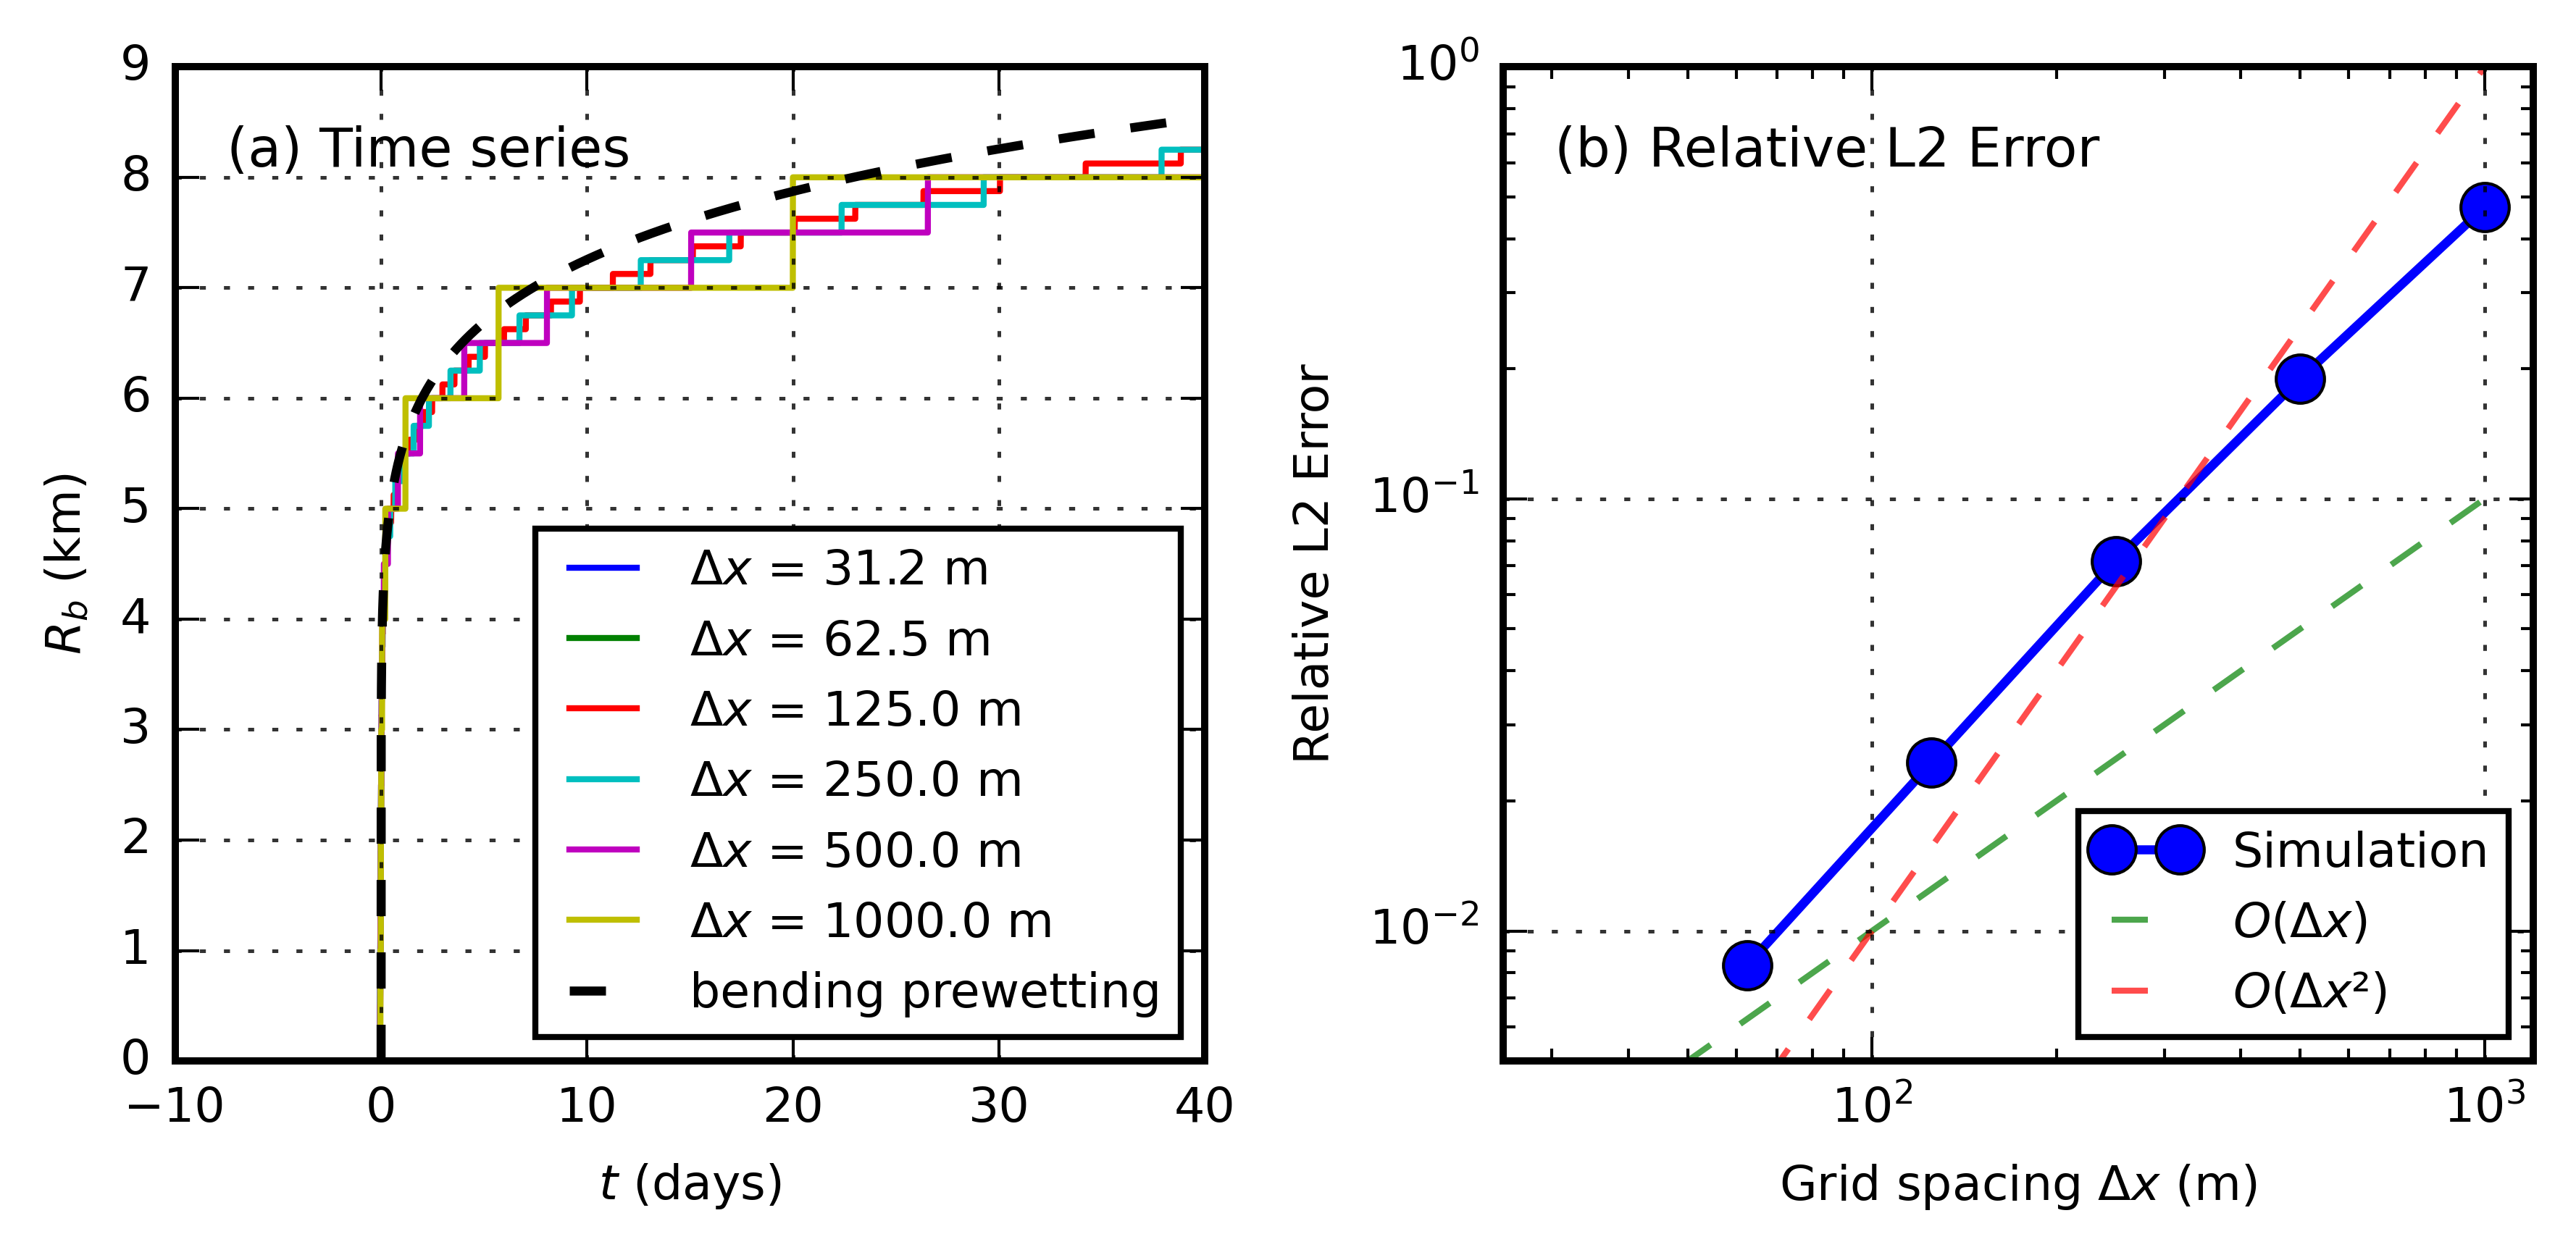
\includegraphics[width=1.0\linewidth]{./figures/Fig9_convergence_1.png}
    \caption{\textbf{Convergence test under a bending-dominated regime.} (\textbf{a}) Time series of the blister radius for different grid sizes $\Delta x$ in the bending-dominated regime. The reference solution is chosen to be the numerical solution with $\Delta x=31.25~\text{m}$. The dashed line is the scaling \eqnref{eq:vel_bending}. (\textbf{b}) The relative error of the blister radius compared to the reference solution as a function of $\Delta x$.}
    \label{fig:convergence_bending_test}
\end{figure}

We have verified that the numerical solution for blister propagation converges as the grid size $\Delta x\rightarrow 0$ by simulating both bending-dominated and gravity-dominated regimes in a one-dimensional model at various grid resolutions. For the bending-dominated regime, we consider an ice sheet of uniform thickness $H=1000~\text{m}$ resting on a flat bed ($b=0$). A blister with a volume of $10^{2}~\text{m}^2$ and an effective viscosity of $\mu_{\text{eff}}=10^{-3}~\text{Pa}~\text{s}$ propagates symmetrically in both directions. We denote the blister front position as $R_b$, which is defined as the distance from the blister centre to the point where the blister thickness drops below $2h_0$.

For the gravity-dominated regime, the ice sheet has the same uniform thickness ($H=1000~\text{m}$) but rests on a linear bedrock slope of angle $\theta=10^{-2}$. The blister has the same volume but a larger effective viscosity of $\mu_{\text{eff}}=10^{1}~\text{Pa}~\text{s}$. In this case, the blister still propagates symmetrically at early times under bending stresses, but eventually shifts to a unidirectional downslope propagation, and we again use $R_b$ to denote the distance travelled by the blister front.

The grid size $\Delta x$ ranges from $1000~\text{m}$ down to $31.25~\text{m}$ in both regimes. The numerical solution obtained at the finest grid resolution, denoted as $R_{b,\text{ref}}$, serves as the reference solution. For a given grid size $\Delta x$, the relative error $E$ of the time series $R_b(t)$ is defined as 
\begin{linenomath*}
\begin{equation}\label{eq:error}
    E\left(R_b\right) = \frac{\Vert R_b\left(t\right)-R_{b,\text{ref}}(t)\Vert}{\Vert R_{b,\text{ref}}(t) \Vert},
\end{equation}
\end{linenomath*}
where $t$ ranges from $0$ to $40$ days, and $\Vert\cdot\Vert$ denotes the $L^2$ norm over time.

\begin{figure}[!ht]
    \centering
    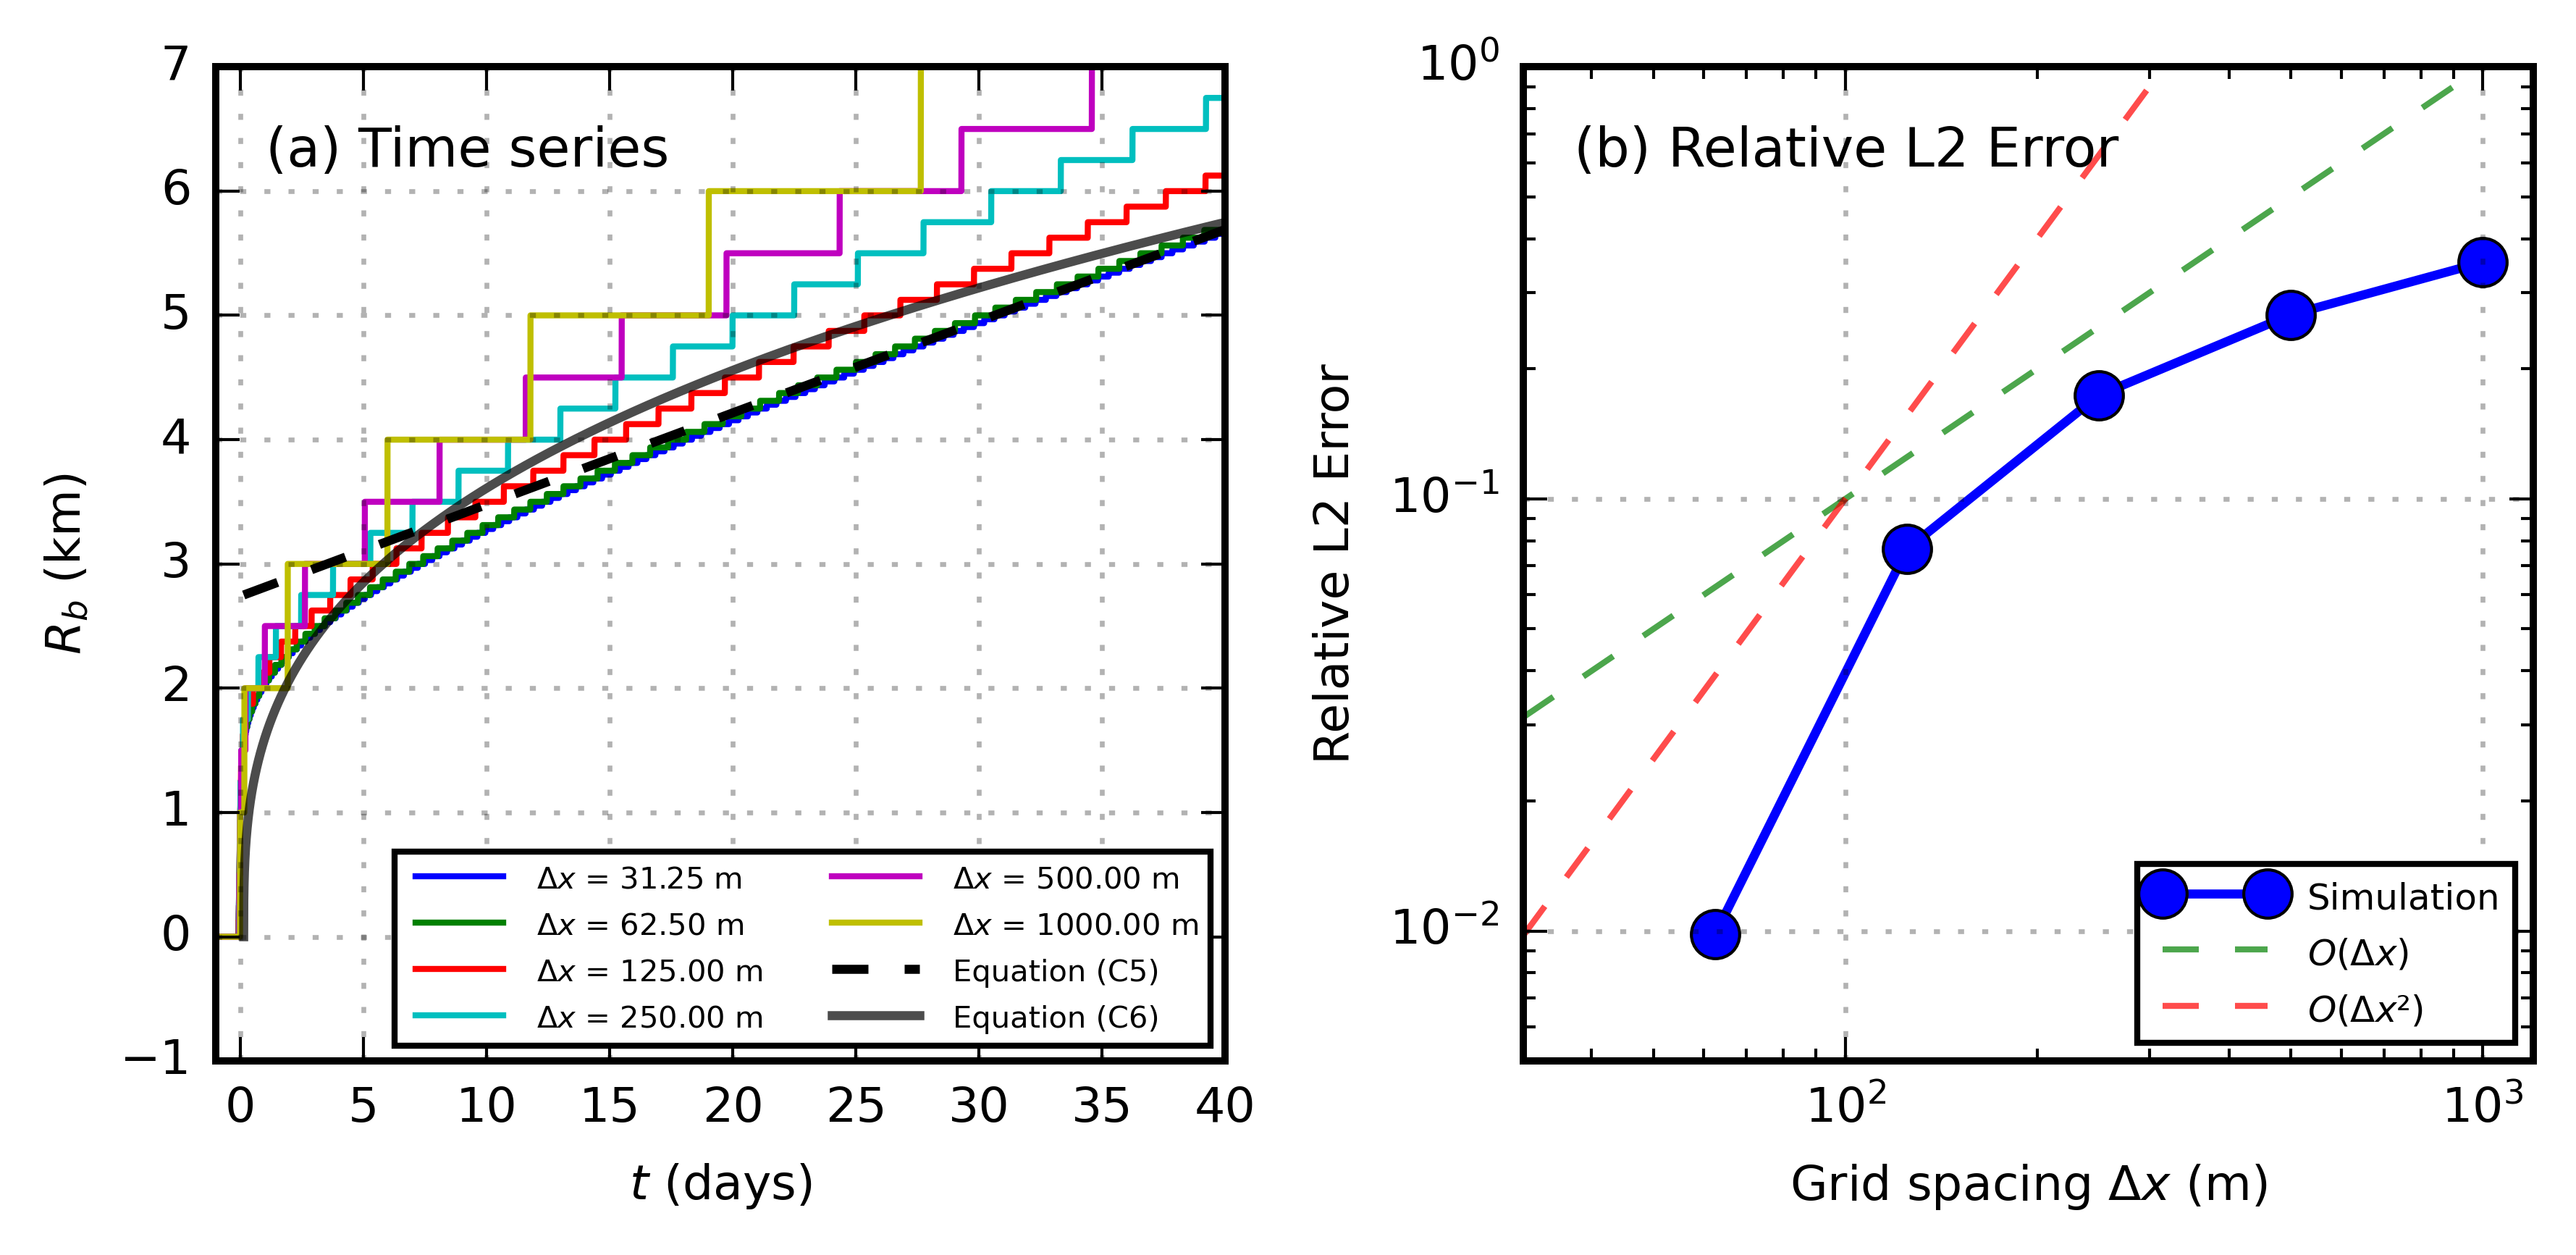
\includegraphics[width=1.0\linewidth]{./figures/Fig10_convergence_2.png}
    \caption{\textbf{Convergence test under a gravity-dominated regime.} (\textbf{a}) Time series of the blister front position for different grid sizes $\Delta x$ in the gravity-dominated regime with a linear bedrock profile with an angle of $\theta=10^{-2}$. The reference solution is chosen to be the numerical solution with $\Delta x=31.25~\text{m}$. The solid black line and the dashed black line are scalings obtained from the scaling for a gravity-dominated blister (\eqnref{eq:vel_gravity_fracture}) and the scaling for a viscous gravity current (\eqnref{eq:vel_gravity}), respectively. (\textbf{b}) The relative error of the blister radius compared to the reference solution as a function of $\Delta x$.}
    \label{fig:convergence_gravity_test}
\end{figure}

The convergence test for the bending-dominated regime is shown in \figref{fig:convergence_bending_test}. The relative error of the blister radius compared to the reference solution decreases as the grid size $\Delta x$ is reduced. The corresponding convergence test for the gravity-dominated regime is presented in \figref{fig:convergence_gravity_test}, where the relative error similarly decreases with decreasing $\Delta x$. Based on these results, we select a grid size of $\Delta x=125~\text{m}$ for the reference cases presented in \secref{sec:results}, and $\Delta x=900~\text{m}$ for the regional study in \secref{sec:regional_study}, as this grid-size choice provides a balance between accuracy and computational efficiency.

\section{Scalings for the blister propagation}\label{apdx:scalings}
Here we summarise the expected scalings for the blister propagation and leakage from previous literature. We focus on axisymmetric blisters with a constant volume $V_b$. The position of the blister front is denoted as $R_b(t)$. 

For the bending-dominated regime \cite{peng2020Viscous}, the propagation velocity $\dot{R_b}$ can be derived as
\begin{linenomath*}
\begin{equation}\label{eq:vel_bending}
    \dot{R_b} = 76.1 \frac{B h_0^{1/2} V_b^{5/2}}{12\mu_{\text{eff}}R_b^{10}},
\end{equation}
\end{linenomath*}
where $B$ is the bending stiffness, and $h_0$ is the pre-wetted layer thickness. Assuming that $R_b=0$ at $t=0$, integrating \eqnref{eq:vel_bending} over $t$ gives the blister radius as
\begin{linenomath*}
\begin{equation}\label{eq:rb_bending}
    R_b = 1.47 \left(\frac{B h_0^{1/2} V_b^{5/2}}{\mu_{\text{eff}}}\right)^{1/11} t^{1/11},
\end{equation}
\end{linenomath*}
which indicates that the dependence of $\dot{R_b}$ on the effective viscosity $\mu_{\text{eff}}$ and the lake drainage volume $V_l$ are relatively weak, with $\dot{R_b}\sim \mu_{\text{eff}}^{-1/11}$ and $\dot{R_b}\sim V_b^{5/22}$ (\figref{fig:blister_velocity}). 

In the one-dimensional geometry used in the convergence test (\appref{apdx:convergence_test}), we use $V_b$ to denote the blister volume per unit width in the cross-slope direction. The scaling for the velocity is
\begin{linenomath*}
\begin{equation}\label{eq:vel_bending_1d}
    \dot{R_b} = 411 \frac{B h_0^{1/2} V_b^{5/2}}{12\mu_{\text{eff}}R_b^{15/2}},
\end{equation}
\end{linenomath*}
and thus for the radius,
\begin{linenomath*}
\begin{equation}\label{eq:rb_bending_1d}
    R_b = 1.95 \left(\frac{B h_0^{1/2} V_b^{5/2}}{\mu_{\text{eff}}}\right)^{2/17} t^{2/17}.
\end{equation}
\end{linenomath*}

For the gravity-dominated regime \cite{tobin2023Evolution}, propagation of the blister can be approximated as one-dimensional (along the downslope direction). In this regime, the front velocity $\dot{R_b}$ is given by
\begin{linenomath*}
\begin{equation}\label{eq:vel_gravity}
    \dot{R_b} = \frac{\left(\rho_w g V_b \sin{\alpha}\right)^{5/4} h_0^{1/2}}{12\mu_{\text{eff}} B^{1/4}},
\end{equation}
\end{linenomath*}
where $\alpha$ is the angle of the bed slope. This scaling indicates that the propagation velocity is constant in time given a constant bed slope. Note that this scaling assumes the blister has propagated sufficiently far donwslope, as gravity effects need to dominate over bending effects. The dependence of $\dot{R_b}$ on the effective viscosity $\mu_{\text{eff}}$ and the lake drainage volume $V_l$ are relatively strong, with $\dot{R_b}\sim \mu_{\text{eff}}^{-1}$ and $\dot{R_b}\sim V_b^{5/4}$ (\figref{fig:blister_velocity}).

Note that our blister model with a pre-wetted layer depends on the regularisation parameter $h_0$.  Alternatively, assuming that the blister is a viscous gravity current propagating on a dry bed \citef{huppert1982Flow}, the scaling of the front speed $\dot{R_b}$ follows a power-law decay controlled by the balance between the downslope component of gravity and viscous forces:
\begin{linenomath*}
\begin{equation}\label{eq:vel_gravity_fracture}
    \dot{R_b} = \frac{1}{2^{2/3}}\left(\frac{\rho_w g V_b^2 \sin{\alpha}}{12\mu_{\text{eff}}}\right)^{1/3}t^{-2/3},
\end{equation}
\end{linenomath*}
thus
\begin{linenomath*}
\begin{equation}\label{eq:rb_gravity_fracture}
    R_b = \frac{3}{2^{2/3}}\left(\frac{\rho_w g V_b^2 \sin{\alpha}}{12\mu_{\text{eff}}}\right)^{1/3}t^{1/3}. 
\end{equation}
\end{linenomath*}

Different from the gravity-dominated blister with a pre-wetted layer, the propagation velocity of a gravity current decays with time (\eqnref{eq:vel_gravity_fracture}). In \figref{fig:convergence_gravity_test}a, we compare the front position $R_b$ of the gravity-dominated blister with a pre-wetted layer to the scaling in \eqnref{eq:vel_gravity} (integrated over time and shifted to match the numerical results at late times) and the scaling in \eqnref{eq:rb_gravity_fracture}. With the choice of $h_0=10^{-3}$ m, the numerically-simulated propagation velocity remains close to the scaling in \eqnref{eq:vel_gravity_fracture} within the simulation time of $40$ days, which justifies our choice of $h_0$ in this study.

%%%%%%%%%%%%%%%%%%%%%%%%%%%%%%%%%%%%%%%%%%%%%%%
%
% DATA SECTION and ACKNOWLEDGMENTS
%
%%%%%%%%%%%%%%%%%%%%%%%%%%%%%%%%%%%%%%%%%%%%%%%
\section*{Open Research Section}
The code used to run the simulations in this study is available at \url{https://github.com/HwenZhang/nevis}, which is a modified version of the subglacial hydrology model by \citeA{hewitt2013Seasonal}. The data used in the regional study in \secref{sec:regional_study} can be downloaded from the following sources: the IceBridge BedMachine Greenland Version 2 \cite{morlighem2014Deeply} at \url{https://nsidc.org/data/idbmg4/versions/2}; the Greenland Ice Mapping Project (GIMP) digital elevation model \cite{howat2014Greenland} at \url{https://nsidc.org/data/nsidc-0645/versions/1}, used by \citeA{stevens2018Relationship} at \url{https://zenodo.org/records/1299945}.

\section*{Conflict of Interest declaration}
The authors declare there are no conflicts of interest for this manuscript.

\section*{Copyright}
For the purpose of open access, the authors have applied a CC BY public copyright licence to any author accepted manuscript arising from this submission.

\acknowledgments
This work was supported by the Natural Environment Research Council (NERC) grant NE/Y002369/1, as a part of the joint NSF-NERC project ``Understanding surface-to-bed meltwater pathways across the Greenland Ice Sheet using machine-learning and physics-based models." The authors thank project members F. Clerc, C.-Y. Lai, E. Lee, J. Rines, and L. Stearns for helpful discussions.

\bibliography{zhang2025subglacial}

\end{document}



